\documentclass[lettersize,journal]{IEEEtran}
\usepackage{amsmath,amsfonts}
\usepackage{algorithmic}
\usepackage{algorithm}
\usepackage{array}
\usepackage[caption=false,font=normalsize,labelfont=sf,textfont=sf]{subfig}
\usepackage{textcomp}
\usepackage{stfloats}
\usepackage{float}
\usepackage{url}
\usepackage{verbatim}
\usepackage{graphicx}
\usepackage{gensymb}
\usepackage{xcolor}
\usepackage{cite}
\usepackage{utfsym}
%\usepackage[justification=centering, font={footnotesize, stretch=2}, labelsep=period]{caption}
\usepackage[font={footnotesize, stretch=1}, labelsep=period]{caption}
% updated with editorial comments 8/9/2021

\begin{document}

\title{LFD-Net: Lightweight Feature-interaction Dehazing Network for Real-time Remote Sensing Tasks}
  
\author{
    Yizhu Jin, Jiaxing Chen, Feng Tian and Kun Hu \IEEEmembership{Member,~IEEE} % <-this % stops a space
    % \thanks{This paper was produced by the IEEE Publication Technology Group. They are in Piscataway, NJ}% <-this % stops a space
    \thanks{Manuscript received May 3, 2023; revised Jun 23, 2023. This work was supported in part by the Institute of Artificial Intelligence, the Youth talent support program of Beihang University under Grant KLSMNR-202208, in part by the National Innovation Center of Intelligent and Connected Vehicles, and in part by the Key Laboratory of Land Satellite Remote Sensing Application, Ministry of Natural Resources of the People's Republic of China under Grant YWF-22-L-1277. \textit{(Corresponding author: Kun Hu.)}}
    \thanks{Kun Hu is with the Institute of Artificial Intelligence, Beihang, China. Yizhu Jin is with the School of Automation Science and Electrical Engineering, Beihang, China (e-mail: kunhu@buaa.edu.cn, 19374316@buaa.edu.cn).}
    \thanks{Jiaxing Chen and Feng Tian are with the National Innovation Center of Intelligent and Connected Vehicles, Beijing, China (e-mail: chenjiaxing@china-icv.cn, fengtianreal95@gmail.com).}
    \thanks{(Yizhu Jin and Jiaxing Chen contributed as co-first authors.)}
}

% The paper headers
\markboth{Journal of \LaTeX\ Class Files,~Vol.~14, No.~8, August~2021}%
{Shell \MakeLowercase{\textit{et al.}}: A Sample Article Using IEEEtran.cls for IEEE Journals}

% \IEEEpubid{0000--0000/00\$00.00~\copyright~2021 IEEE}
% Remember, if you use this you must call \IEEEpubidadjcol in the second
% column for its text to clear the IEEEpubid mark.

\maketitle

\begin{abstract}
Currently, remote sensing equipments are evolving towards intelligence and integration, incorporating edge computing techniques to enable real-time responses. One of the key challenges in enhancing downstream decision-making capabilities is the pre-processing step of image dehazing. Existing dehazing methods usually suffer from steep computational costs with densely connected residual modules, as well as difficulties in maintaining visual quality. To tackle these problems, we designed a lightweight Atmosphere Scattering Model (ASM) based network structure to extract, fuse and weight multiscale features. Our proposed LFD-Net demonstrates strong interpretability by exploiting the gated fusion module and attention mechanism to realize feature interactions between multi-level representations. The experimental results of LFD-Net on SOTS dataset reach an average Frequency Per Second (FPS) of 54.41, approximately 8 times faster than seven most popular SOTA methods with equivalent metrics. After image dehazing by LFD-Net, the performance of object detection is significantly improved. The mean Average Precision when IoU = 0.5 (mAP@0.5) based on YOLOv5 is improved by 4.73\% on DAIR-V2X dataset, which verified the practicability and adaptability of LFD-Net for real-time vision tasks. Our codes are available at {\color[HTML]{DD00DD} \texttt{\url{https://github.com/RacerK/LFD-Net}}}.
\end{abstract}

\begin{IEEEkeywords}
single image dehazing, real-time application, model compression, interpretablity.
\end{IEEEkeywords}

\section{Introduction}
\IEEEPARstart{R}{emote} \textcolor{blue}{sensing refers to the process of collecting information or data about an object, area, or phenomenon from a distance, typically using sensors mounted on aircraft, satellites, or other platforms~\cite{lillesand2014remote}.} Nowadays, the construction of space-air-ground integrated remote sensing land observation networks is of great importance for various industrial applications~\cite{li2020nasa, tam2021adaptive}. Based on platforms such as satellites, aircraft, drones, vehicles, and ground monitoring devices, one can obtain comprehensive information about ground objects. However, real-time accurate information extraction in complex and highly dynamic conditions, such as traffic regulation, crime tracking, and disaster relief, remains particularly difficult~\cite{zheng2022dehaze, han2021edge, makarau2014haze}. A key pre-processing step to improve image quality is to remove the negative effects of prevailing haze, and it would be a good option to deploy dehazing algorithms on remote sensing terminal platforms, which could significantly reduce data transmission costs and achieve fast response. Therefore, it is necessary to propose a lightweight dehazing algorithm to remove the constraints of limited power and computing resources on edge devices, and optimize the dehazing efficiency while ensuring accuracy and reliability.

\begin{figure}[t]
    \centering
    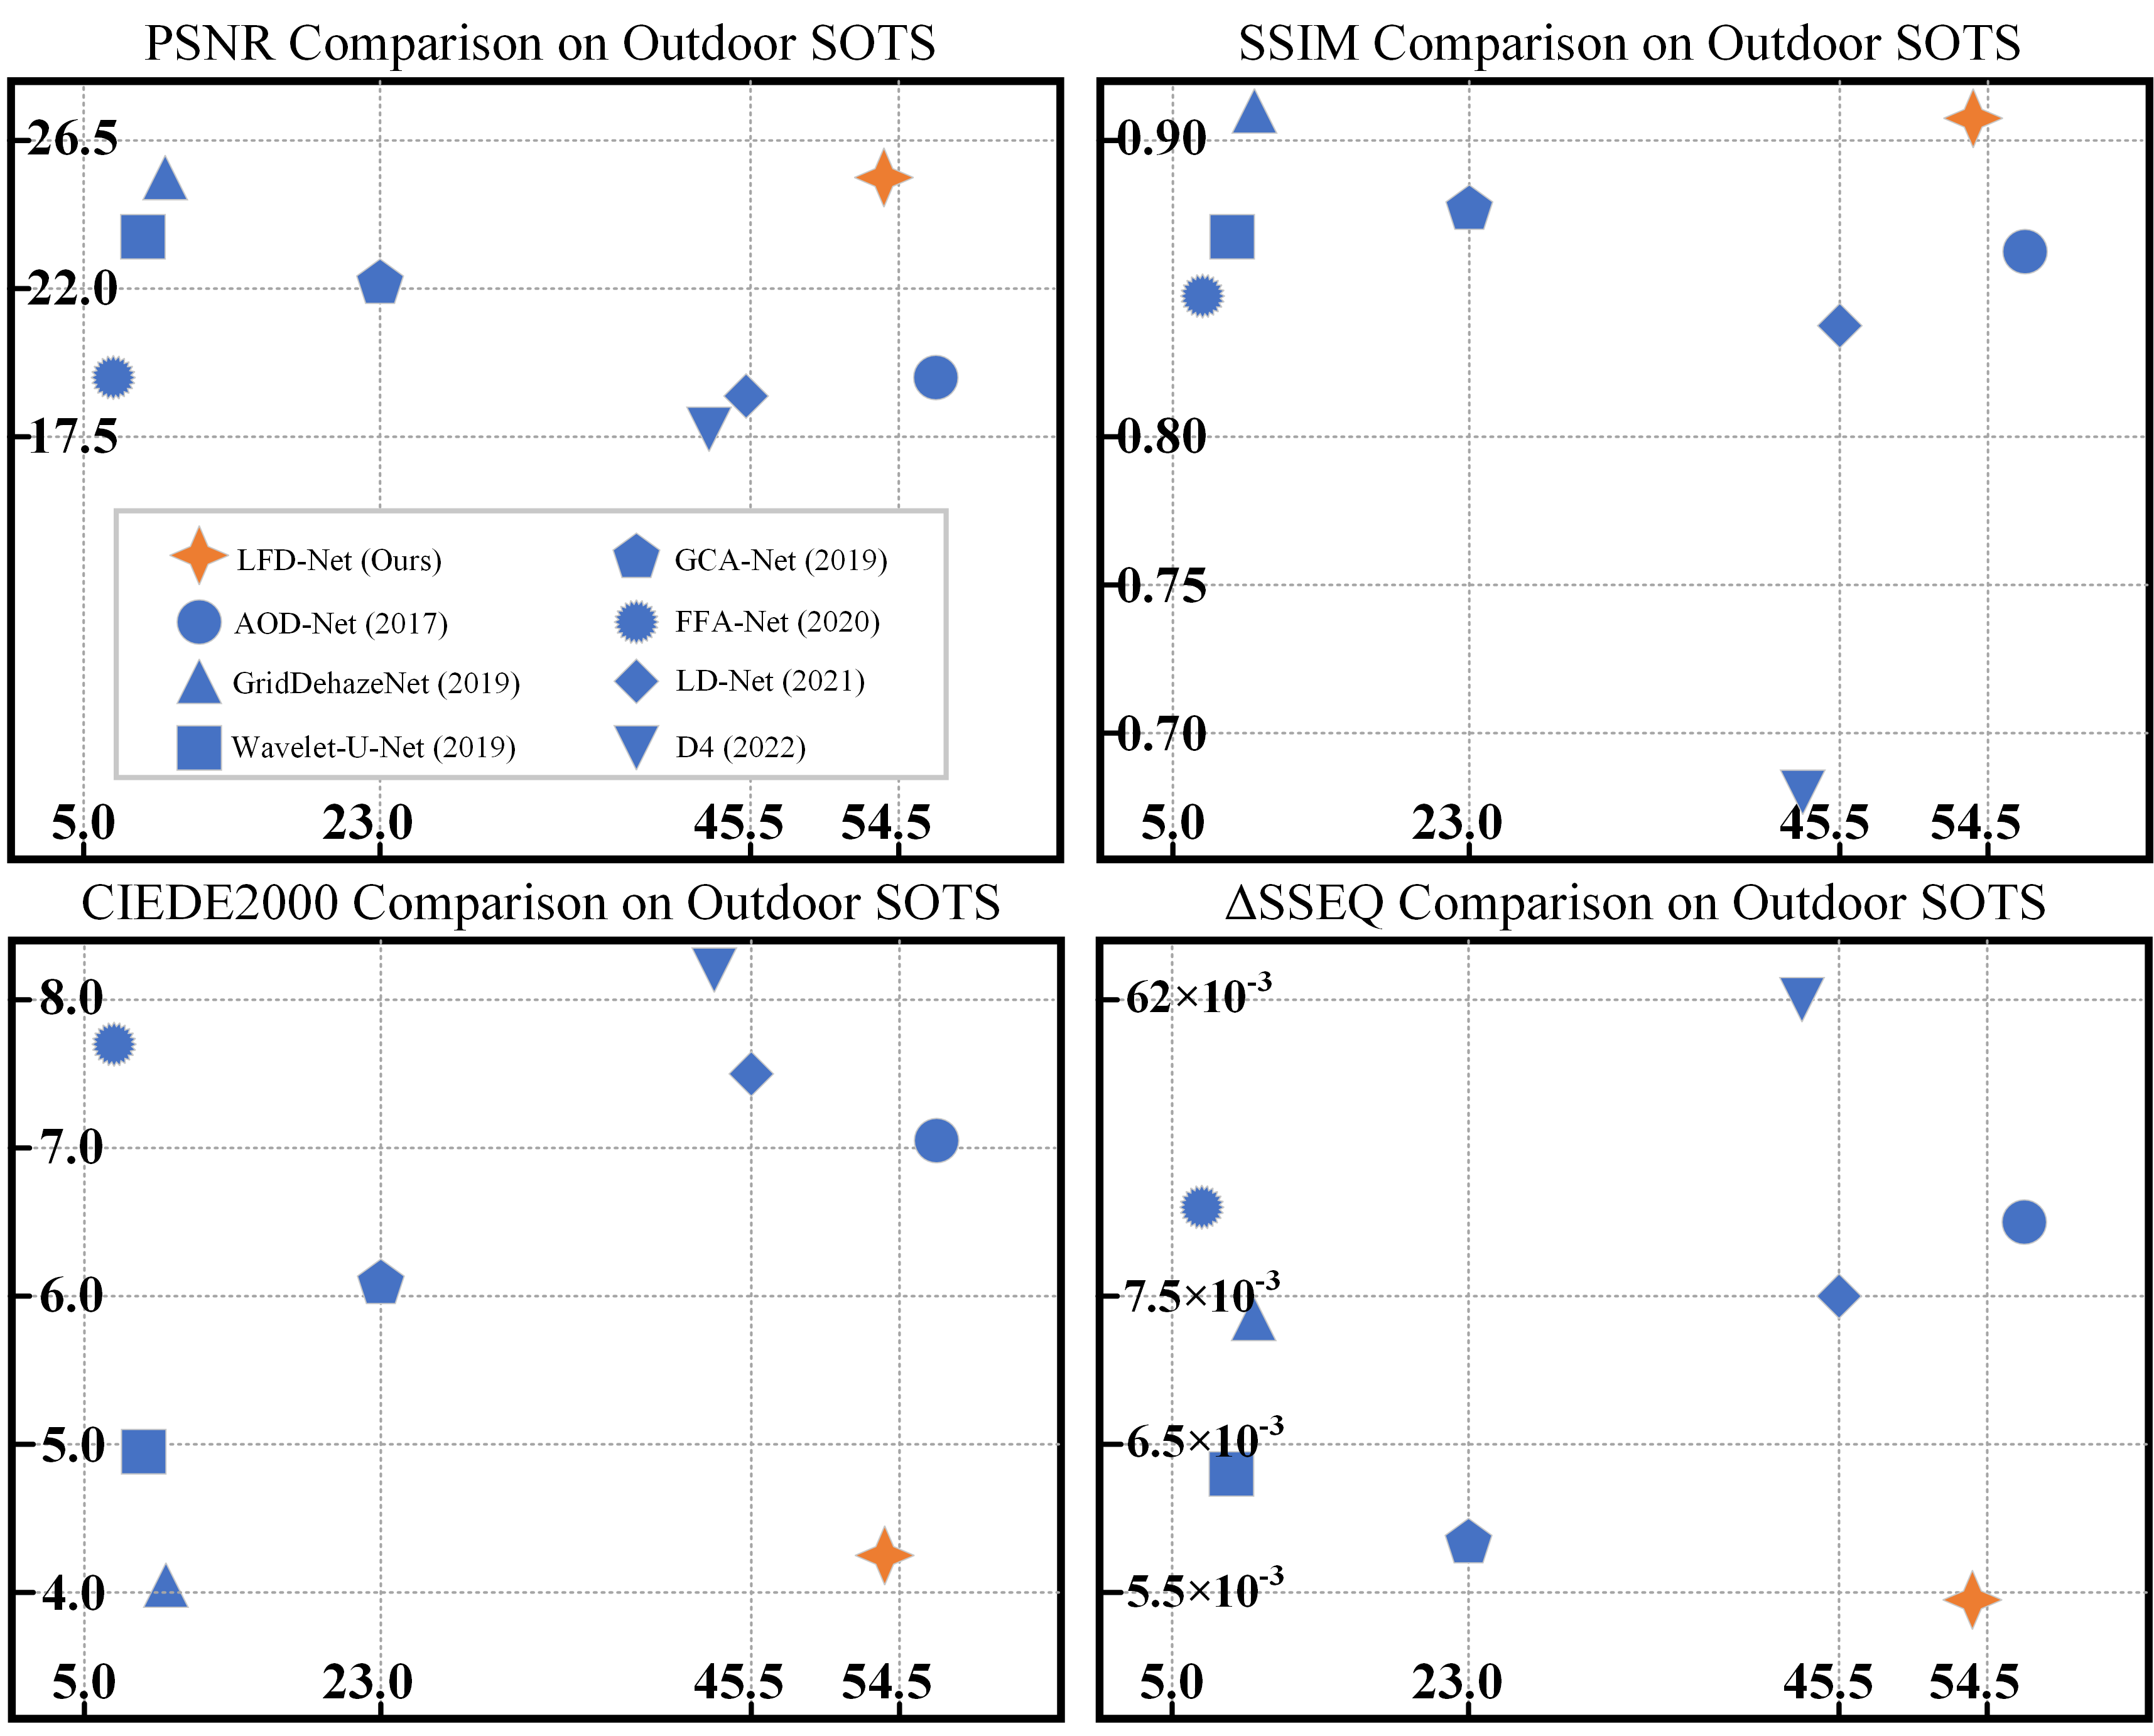
\includegraphics[width=8.5cm]{sample.png}
    \caption{Comparison Metrics on Outdoor SOTS, in terms of PSNR, SSIM, CIEDE2000, $\Delta$SSEQ ($\uparrow$) and FPS ($\rightarrow$).}
    \label{sample}
\end{figure}

% Therefore, if remote sensing data processing is partially performed on the drone or satellite platform, the transportation of effective information could alleviate the stress on earth-based servers and enable more prompt responses to emergency situations. Additionally, drones and satellites are typically considered edge devices with limited power and computing resources due to strong demands from engines or monitors~\cite{ma2021light, tam2021adaptive}. As a result, the processing algorithms need to be designed to efficiently use these limited resources while still producing accurate results. An effective and efficient dehazing approach is urgently needed for edge computing and remote sensing applications to mitigate the impact of haze on image quality and accuracy, which could potentially revolutionize the way we utilize remote sensing data for various applications.

Dehazing methods for remote sensing images are mainly of three types: prior knowledge based methods, physical model based methods, and deep learning based methods. Most of the earliest dehazing methods are based on prior knowledge. For instance, Dark Channel Prior makes an approximation that haze-effected pixels have at least one relatively low intensity value among RGB channels~\cite{li2020nasa};  a semi-physical guided-filter based approach is adopted to refine the coarse haze thickness map to restore textural information~\cite{liu2021semiphysical}; depth estimation and image segmentation are incorporated with Dark Channel Prior to generate the final transmittance~\cite{xie2021image}. These prior knowledge based methods are typically subject to empirical or statistical regularities, leading to limited application scenarios.

In addition, ASM has been extensively introduced in physics model based dehazing methods. It is physically-grounded for an unrestricted access to various image scenes through the estimation of global atmosphere light and transmission map. For instance, an end-to-end DehazeNet combines dark channel, maximum contract, color attenuation as well as hue disparity prior to compute the transmission map and assigns a default value to atmosphere light~\cite{cai2016dehazenet}; a Haze Density Prediction Network is designed for a more accurate approximation of atmosphere light to better fit for nighttime occasions~\cite{liao2018hdp}; a multi-decoder framework is presented to handle multiple bad weather restoration, with rain veiling effect embedded into the conventional ASM~\cite{li2020all}, and a differential guided layer is embedded with the backbone and substituted to the physical scattering equation~\cite{li2020all}. Approaches based on ASM are usually more lightweight, but they may produce unnatural color tones due to inaccurate estimation of atmospheric light.

Compared with traditional dehazing methods, deep learning based methods gradually become the research hotspot due to their stronger modeling and generalization capabilities.  Dehazing methods based on Convolutional Neural Networks (CNNs) are extensively adopted, which will be discussed in detail in Section \ref{sec:2}.  %The trade-off between high performance on particular datasets and generalization to diverse practical applications is a central challenge that requires holistic consideration in the design and evaluation of image restoration algorithms. While most current methods may demonstrate promising results under certain conditions, their lack of efficiency and generalization capabilities make them less suitable for real-world and real-time applications. The study of lightweight dehazing methods has become increasingly crucial due to the urgent need for context-aware and fast-response remote sensing systems. For instance, AOD-Net~\cite{li2017aod} strives to concatenate multi-level features in different patterns, which is the baseline of other lightweight dehazing models. Both FAOD-Net~\cite{2020FAOD} and GADO-Net~\cite{GAOD} introduce depth-wise, point-wise convolution to reduce the amount of parameters and aggregate context information in pyramid pooling module. FAMED-Net~\cite{2020FAMED} applies cascaded and densely connected point-wise convolutional and pooling layers at three scales. LD-Net~\cite{ullah2021light} concatenates convolutional layers that have a semantic gap rather than combining adjacent layers and leverages a Color Visible Restoration module to improve the color consistency.

% To address the issue of haze in remote sensing, researchers have developed various methods to dehaze the images, including the use of image priors, physical models and deep learning techniques. These methods aim to remove the effects of haze from the images to improve their clarity and detail, thereby enhancing the accuracy of high-level perception tasks. 

% The earliest dehazing methods are mainly based on prior knowledge. For instance, in\cite{he2010single}, Dark Channel Prior makes an approximation that haze-effected pixels have at least one relatively low intensity value among RGB channels. 

% In\cite{liu2021semiphysical}, a semi-physical guided-filter based approach is adopted to refine the coarse haze thickness map to restore textural information. In\cite{xie2021image}, depth estimation and image segmentation are incorporated with Dark Channel Prior to generate the final transmittance. Generally, these methods are subject to empirical or statistical regularities, which limits the application scenarios to some extent.

% Furthermore, as a physic-based model, ASM is also extensively researched and introduced in dehazing methods. It is physically-grounded for an unrestricted access to various image scenes through the estimation of global atmosphere light and transmission map. For instance, in \cite{cai2016dehazenet}, an end-to-end DehazeNet combines dark channel, maximum contract, color attenuation as well as hue disparity prior to compute the transmission map and assigns a default value to atmosphere light. In \cite{liao2018hdp}, a Haze Density Prediction Network is designed for a more accurate approximation of atmosphere light to better fit for nighttime occasions. In \cite{li2020all}, a multi-decoder framework is presented to handle multiple bad weather restoration, with rain veiling effect embedded into the conventional ASM. In \cite{li2020all}, a differential guided layer is embedded with the backbone and substituted to the physical scattering equation.

% In addition to traditional dehazing methods, deep learning techniques have been widely adopted in dehazing research. Among these techniques, Convolutional Neural Networks (CNNs) have been the most extensively studied architecture for deep-learning-based dehazing methods. In our method, we also use CNNs as the underlying architecture. In the second section, we will discuss the common challenges and techniques in developing CNN-based dehazing methods.

% In addition to traditional dehazing methods, deep learning techniques have been widely adopted in dehazing research. Among these techniques, Convolutional Neural Networks (CNNs) have been the most extensively studied architecture for deep-learning-based dehazing methods. In our method, we also use CNNs as the underlying architecture. In the second section, we will discuss the common challenges and techniques in developing CNN-based dehazing methods. Besides CNNs, Generative Adversarial Networks (GANs) have also been applied in image dehazing. For example, in \cite{guo2020joint}, an integrated multi-task algorithm is proposed to jointly remove raindrop and haze from both sky and non-sky regions. In \cite{li2020deep}, the generator is designed to capture uneven foggy features in sequential and parallel manners to obtain haze-free images. In \cite{ding2021perceptual}, an inverse-reverse module is utilized to correlate diverse image styles in adversarial training. In \cite{2019AttentionGAN}, unpaired clean and hazy images are utilized for training, and attention-guided generators produce attention masks, which are fused with generation outputs to enhance image quality. These GAN-based methods perform well on synthetic image data, but they may suffer from a loss of authenticity when applied to natural hazy images. Therefore, our method, which is CNN-based, may be more appropriate for dehazing natural hazy images.

% In deep-learning-based techniques, there is a persistent challenge of the trade-off between high performance on specific datasets and generalization to diverse real-world applications. It is crucial to consider both performance and generalization when developing and evaluating potential solutions in image restoration. Although current methods may demonstrate promising results under certain conditions, their lack of efficiency and generalization capabilities render them less suitable for real-time and practical applications. Due to the urgent need for a context-awareness system supporting quick response confronted with extreme situations, the study of lightweight dehazing methods has become increasingly crucial. AOD-Net\cite{li2017aod} strives to concatenate multi-level features in different patterns, which is the baseline of other lightweight dehazing models. Both FAOD-Net\cite{2020FAOD} and GADO-Net\cite{GAOD} introduce depth-wise, point-wise convolution to reduce the amount of parameters and aggregate context information in pyramid pooling module. FAMED-Net\cite{2020FAMED} applies cascaded and densely connected point-wise convolutional and pooling layers at three scales. LD-Net\cite{ullah2021light} concatenates convolutional layers that have a semantic gap rather than combining adjacent layers. Besides, it leverages a Color Visible Restoration module to improve the color consistency. 

% Our proposed Lightweight Feature-interaction Dehazing Network (LFD-Net) utilizes a cascade of convolutional layers, while focusing on the interaction of multi-level features. We adopt a feature-fusion module that uniformly takes in multi-level features generated by the cascaded convolutional layers with different kernel sizes. Besides, attention mechanism is also applied to adaptively learn the weights of inter- and intra-channel features and selectively contribute to more conducive image levels or regions. Overall, our main combinations are three-fold:

Our proposed Lightweight Feature-interaction Dehazing Network (LFD-Net) utilizes convolutional layers of different kernel sizes as a sequence to extract multi-level features. The feature interaction process is addressed coherently by taking in, redistributing, and reassigning weights to the extracted features. Each component of our network performs its own function, but also interacts efficiently and effectively as a whole. Moreover, we utilize multiple metrics for evaluation, which are highly relevant and sensitive to remote sensing tasks. Overall, our main contributions are threefold:

\begin{itemize}
    \item[$\bullet$] Our method employs ASM to jointly approximate atmospheric light and transmission maps to enhance image restoration capability and inference efficiency. It incorporates the convolutional operations into more specialized modules while maintaining the conciseness.
    \item[$\bullet$] Our proposed method is designed to provide interpretability by assigning distinct tasks to each module, as demonstrated by the results of our visualization and ablation experiments. The feature-interaction process relies heavily on element-wise multiplication, which has been shown to enhance the performance of pure convolutional operations.
    % We propose a novel framework with a progressive feature extracting process, during which multi-level representations are interconnected by Gated Fusion Module with a proceeding Attention Mechanism. Complicated design of architecture or stack of sophisticated modules is avoided in our method to reduce parameters. We also conduct adequate ablation study to demonstrate the indispensability of each component in our network. 
    \item[$\bullet$] Our proposed method has been extensively validated across various scenarios of space-air-ground remote sensing land observation tasks to demonstrate its stability, practicality, and generalization capabilities. It can effectively address common challenges such as halo effects, gridding artifacts, and color inconsistency, and achieves an excellent trade-off between accuracy and efficiency, which considerably improves the performance of object detection.
    %Our proposed method has been extensively validated across various scenarios across sky, earth and space, to demonstrate its stability, practicality, and generalization for integral remote sensing tasks, achieving an excellent trade-off between accuracy and efficiency. Our approach effectively addresses common challenges such as halo effect, gridding artifact, and color inconsistency, resulting in significant improvements in the performance of object detection tasks.

\end{itemize}

\section{Related Work}
\label{sec:2}

\textcolor{blue}{The increasing prevalence of intelligent remote sensing devices that support real-time responses, as opposed to relying on data transmission to servers, has highlighted the importance of studying lightweight dehazing methods, which are crucial for context-aware and fast-response remote sensing systems. However, there exists a trade-off between the efficiency and accuracy of lightweight dehazing approaches. Some approaches employ knowledge distillation~\cite{hong2020distilling, suresh2022rich} or pruning techniques~\cite{liu2022aerial}, which may sacrifice accuracy for efficiency. In contrast, other methods directly construct lightweight networks to address this issue. For instance, AOD-Net~\cite{li2017aod} serves as a baseline for other lightweight dehazing models by concatenating multi-level features using different patterns. FAOD-Net~\cite{2020FAOD} and GAOD-Net~\cite{GAOD} utilize depth-wise and point-wise convolutions to reduce parameters and aggregate context information in a pyramid pooling module. FAMED-Net~\cite{2020FAMED} employs cascaded and densely connected point-wise convolutional and pooling layers at multiple scales. LD-Net~\cite{ullah2021light} tackles the semantic gap by concatenating convolutional layers and incorporates a Color Visible Restoration module to enhance color consistency.}

\textcolor{blue}{Nevertheless, achieving a balance between high performance on specific datasets and generalization to diverse practical applications remains a central challenge. The design and evaluation of dehazing methods should consider this trade-off comprehensively. While current methods may exhibit promising results under certain conditions, their lack of efficiency and generalization capabilities limit their suitability for real-world and real-time applications.} 

Our proposed LFD-Net considers dehazing as an image reconstruction task with an emphasis on feature extraction and feature utilization processes, as discussed in Section \ref{subsec:2.1} and \ref{subsec:2.2}. \textcolor{blue}{In contrast to stacking deep residual modules in these procedures, we employ the gated fusion and attention mechanism only once, which improves both efficiency and interpretability.} Moreover, it is important to design comprehensive evaluation metrics for dehazing methods, as described in Section \ref{subsec:2.3}. 

\subsection{Feature Extraction}
\label{subsec:2.1}
One of the key challenges in image reconstruction is the extraction of multi-level or multi-scale features, which can be facilitated by using a symmetric encoder-decoder structure. The U-Net architecture, originally designed for effective extraction of context information at different scales or levels \cite{ronneberger2015u}, has been widely used as a backbone in various reconstruction tasks. In \cite{dong2020multi}, the Strengthen-Operate-Subtract boosting strategy is incorporated into the decoder, and a dense feature fusion module utilizing a back-projection feedback scheme is leveraged to compensate the missing spatial information from high-resolution features. In \cite{yang2019wavelet}, the U-Net architecture is modified to incorporate discrete wavelet transform and inverse discrete wavelet transform in place of conventional down-sampling and up-sampling. In \cite{feng2021urnet}, hybrid convolution is applied in the U-Net encoder, which combines standard convolution with dilated convolution, to expand the receptive field and extract image features with more detail.

As opposed to a fixed backbone like U-Net, some methods utilize more flexible structures with multiple paths to diversify color information or perform various tasks. For instance, in \cite{lee2020cnn}, image dehazing and depth estimation are addressed simultaneously in a framework with four decoders sharing information from the same encoder. In \cite{li2021underwater}, a multi-color space encoder that incorporates RGB, LAB, and HSV is applied to extract representative features in separate paths. In \cite{mehra2020reviewnet}, quadruple color-cue is integrated into a multi-look architecture with multi-weighted training loss for autonomous vehicular application. These color spaces are often designed manually, which may work well for specific applications, but lack adaptability and generalization.

% Overall, in spite of a diversity of features extracted in multiple paths, it is still challenging for the corresponding feature integration operations, which might reduce the convergence of the models with limited generalization.

\subsection{Feature Utilization}
\label{subsec:2.2}
Another major challenge in image reconstruction tasks is the efficient utilization of extracted features, which has prompted the exploration of various feature fusion strategies and attention mechanisms. For instance, in \cite{liu2019griddehazenet}, a novel attention-based multi-scale estimation module is implemented in the backbone on a grid network to alleviate the bottleneck issue encountered in conventional multi-scale approaches. In \cite{qin2020ffa}, a block structure integrated with Channel-wise Attention (CA), Pixel-wise Attention (PA) is stacked to form a group structure, which is progressively triple-stacked and concatenated to feed into another CA-PA attention mechanism for feature fusion. In \cite{zhang2020multi}, a multi-level fusion module is presented to integrate low-level and high-level representations. In addition, a Residual Mixed-convolution Attention Module is developed to guide the network to focus on significant features during the learning process. In \cite{2022selfguided}, the feature fusion method progressively aggregates the features of hazy image and generated reference image to remove the useless features.

Moreover, the self-attention mechanism proposed in Transformer has also been practiced in dehazing methods. For instance, a Transformer-based channel attention module and a spatial attention module are combined to form an attention module that enhances channel and spatial features\cite{gao2022novel}. Long-range dependencies of image information can be effectively extracted through Transformer blocks in image dehazing\cite{yang2022mstfdn}. Recently, it has been revealed in \cite{rao2022hornet} that self-attention mechanism inherently functions as a two-order feature interaction. Based on this, gated convolution has been developed as an alternative method to achieve an competitive results to self-attention, while reducing the computational cost. 

\subsection{Quality Evaluation}
\label{subsec:2.3}
Existing methods usually focus on high performance quantified by metrics in terms of peak-signal-to-noise-ratio (PSNR) and structure similarity index (SSIM). More specifically, PSNR measures the ratio between the maximum possible value of a pixel and the power of corrupting noise that affects the restoration fidelity. Instead of directly estimating absolute error, SSIM reveals inter-dependencies within pixels by luminance masking and contrast masking between spatially-close image pairs. Besides, CIE2000 Delta E formula (CIEDE2000) and Spatial-Spectral Entropy-based Quality (SSEQ) are also introduced in our comparison metrics, because color and texture are significance for object recognition and terrain classification of remote sensing applications. CIEDE2000 is used to quantify the visual difference between two colors. It takes into account the chromaticity and luminance of the colors being compared, as well as the surrounding colors and the viewing conditions \cite{luo2001ciede2000}. SSEQ is calculated by separating the image into its spatial and spectral components, calculating and combining the entropy of each component\cite{liu2014sseq}. Halo effects in many remote sensing images can lead to significant degradation over large areas compared to high spatial resolution close-range images. In the comparison experiments, we calculate the average CIEDE2000 of each pixel in image pairs and the average absolute value of relative error on SSEQ (\textit{i.e.} $\Delta$SSEQ). 

\section{Proposed Method}
\subsection{Preliminaries}
ASM is employed in our method to overcome the difficulty of raw pixel prediction from reconstructed images via light model. It is physics-based, more suitable for real-world scenarios, and less prone to overfitting during training. The conventional ASM can be reformulated to jointly estimate the global atmosphere light $A$ and the transmission map $t$, resulting in a reduction of parameters \cite{li2017aod}:

\begin{equation}
    \label{deqn_ex1}
    I(\theta) = J(\theta) \times t(\theta) + A(1 - t(\theta)),
\end{equation}
where $A$ is treated as a constant, $t\in (0,1]$ denotes the pixel-wise transmittance of light, $\theta$ represents the pixel coordinate of an $H \times W$ image of height $H$ and width $W$, with $I$ and $J$ being the hazy input and haze-free output, respectively. Therefore, the haze-free approximation $J(\theta)$, can be written as:

\begin{equation}
    \label{deqn_ex2}
    J(\theta) = \frac{I(\theta) - A}{t(\theta)} + A.
\end{equation}

To encapsulate these two factors (\textit{i.e.} $A$ and $t(\theta)$) into one variable, the formula of the reformulated ASM is as follows:

\begin{equation}
    \label{deqn_ex3}
    J(\theta) = K(\theta) \times I(\theta) - K(\theta) + b,
\end{equation}
where $K(\theta)$ represents the new incorporated variable, which can be derived as:

\begin{equation}
    \label{deqn_ex4}
    K(\theta) = \frac{\frac{1}{t(\theta)} \times (I(\theta) - A) + (A - b)}{I(\theta) - 1}.
\end{equation}

To be specific, $K$ is the intermediate evaluation parameter of the network. The ultimate goal is to generate a separate $K$ value for each input channel, typically in terms of RGB. That is, $K$ in size $3 \times H \times W$ is substituted into equation (\ref{deqn_ex3}) at the end of the network, with a most commonly used default value $b = 1$.

\subsection{Network Design}
The proposed LFD-Net distinguishes itself from both heavyweight and lightweight frameworks with its concise and effective approach to feature extraction and interaction, as shown in Fig. \ref{sample}. % In contrast to many existing methods, our network uses the Gated Fusion module and attention mechanism only once, rather than incorporating them as parts of more complex blocks, which contributes to the network's overall lightweight architecture. This design choice allows for efficient processing while maintaining strong performance in dehazing tasks.
To optimize the lightweight structure design of the LFD-Net, the Gated Fusion module and attention mechanism are used only once, instead of incorporating them as parts of more complex blocks. This approach significantly improves efficiency while maintaining strong performance in dehazing tasks.

In CNNs, convolution kernels of varying sizes are used to extract features at different levels of abstraction. Specifically, smaller size kernels are effective at capturing local features, while larger size kernels are more suited for capturing features with larger receptive fields, which are considered as more global features. The most commonly used kernel size is $3 \times 3$. %However, it is not effective enough to stack convolutional layers with this typical kernel size in lightweight models. The utilization of concatenation layers is to combine the low- and high-level features, which compensates for the loss of information from initial layers as the network proceeds deeper. Therefore, the formation of convolutional and concatenation layers are crucial and can be flexibly designed to meet with specific needs. In our proposed method, we benefit from this design concept. Different from existing methods, we further simplify the formation of convolutional layers in feature extracting process. We also introduce feature-interaction strategies as opposed to merely using convolutional and concatenation layers, including the Gated Fusion Module and attention mechanism. 
However, stacking convolutional layers with this typical kernel size is not efficient enough in lightweight models. The concatenation layers are utilized to combine the low-level and high-level features, which compensates the loss of information from the initial layers as the network proceeds deeper. Therefore, the formation of convolutional and concatenation layers is crucial and needs to be designed flexibly to meet specific needs. Different from existing methods, we further simplify the formation of convolutional layers during feature extraction. Based on this, we also introduce feature interaction strategies including the Gated Fusion Module and attention mechanism.

To be specific, in feature extraction, a sequence of convolutional layers with ascending kernel sizes is implemented, ranging from $3 \times 3$, $5 \times 5$ to $7 \times 7$, namely \textit{Conv 1}, \textit{Conv 2} and \textit{Conv 3}. % A residual connection is utilized between \textit{Conv 1} and \textit{Conv 3} to refine the characteristic representations between low- and high-level features.
A residual connection between \textit{Conv 1} and \textit{Conv 3} is utilized to refine feature representations between low-level and high-level features.

\begin{figure*}[t]
    \centering
    \includegraphics[width=\textwidth]{figure1_x.jpg}
    \caption{Architecture of the Lightweight Feature-interaction Dehazing Network. The reformulated ASM generates an explicit output by substituting the evaluated K value. The network primarily consists of convolutional layers and concatenation layers, with the use of element-wise product in the Gated Fusion module and attention mechanism.}
    \label{LFD-Net}
\end{figure*}

A concatenation layer, namely \textit{Concat 1}, is applied to combine the multi-level features from the extraction process. These features are then fed into the Gated Fusion module for spatial interactions, which includes a convolutional operation, namely \textit{Conv 4}. The output features are passed to the second concatenation layer, namely \textit{Concat 2}, which progressively integrates the features extracted in \textit{Conv 3} layer. This is because higher-level information is always more global, and thus being distributed to lower levels in the Gated Fusion module while performing feature interactions. This information is also indispensable for image restoration, especially for the following attention mechanism, which makes it necessary to involve the \textit{Concat 2} layer. The attention mechanism adaptively learns channel-wise and pixel-wise weights to enhance conducive features. After that, all features are fed into the high-resolution stage, which consists of two convolutional layers, namely \textit{Conv 5} and \textit{Conv 6}, respectively. The details of the proposed method are illustrated in Table \ref{tab:table1}.

\begin{table}[pth]
    \caption{Details of the LFD-Net architecture\label{tab:table1}}
    \centering
    \begin{tabular}{ccccc}
    \hline
      & Kernel Size & Stride & Padding & Channel (In / Out)\\
    \hline
    \textit{Conv 1} & 3 & 1 & 1 & 3 / 32\\
    \textit{Conv 2} & 5 & 1 & 2 & 32 / 32\\
    \textit{Conv 3} & 7 & 1 & 2 & 32 / 32\\
    \textit{Concat 1} &
    \multicolumn{4}{c}{\textit{Conv 1}, \textit{Conv 2}, \textit{Conv 1 + Conv 3}}\\
    \textit{Conv 4} & 3 & 1 & 1 & 96 / 3\\
    \textit{Concat 2} &
    \multicolumn{4}{c}{\textit{Conv 3}, The Output of Gated Fusion module}\\
    \textit{Conv 5} & 3 & 1 & 1 & 64 / 16\\
    \textit{Conv 6} & 1 & 1 & 9 & 16 / 3\\
    \hline
    \end{tabular}
\end{table}

\subsection{Gated Fusion Module}
Our proposed LFD-Net replaces densely connected residual blocks with effective feature-interaction based strategies. The Gated Fusion module aims to perform two-order interactions among multi-level features This idea is demonstrated in Transformer-based architecture through two successive pixel-wise product (i.e. $K$, $V$)~\cite{vaswani2017attention}. While Transformers are effective, the computational cost is huge when dealing with low-level preprocessing tasks. Transformer-ensembled CNNs usually expand the flexibility of convolutional operations through adding dynamic weights to improve the modeling power of convolution~\cite{hu2018squeeze, chen2020dynamic, rao2022hornet}. Similar techniques have been practiced in image dehazing methods~\cite{ren2018gated, chen2019gated} but are still in need of further exploration and interpretation. 

Our proposed method also takes advantage of pixel-wise multiplication by directly implementing it to successive feature levels, the concatenation layer \textit{Concat 1} that combines the sequence of convolutional layers \textit{Conv 1}, \textit{Conv 2} and \textit{Conv 3}. For illustration, these features are denoted as $\mathcal{F}_1$, $\mathcal{F}_2$ and $\mathcal{F}_3$ respectively. In addition, these three convolutional operations are denoted as $\mathcal{C}_1$, $\mathcal{C}_2$ and $\mathcal{C}_3$, and the \textit{i}-th feature map of the output layer is denoted as $\mathcal{G}_i$. The process of Gated Fusion module can be expressed mathematically as follows:

\begin{equation}
    \label{deqn_ex5}
    \begin{aligned}
        \mathcal{G}_i &= \sum_{k=1}^3 \mathcal{C}_k(\mathcal{F}) \otimes \mathcal{F}_{k,i}\\
        &= \sum_{k=1}^3 \mathcal{C}_k(\mathcal{F}_{k,i} \oplus \sum_{j \neq i} \mathcal{F}_{k,j}) \otimes \mathcal{F}_{k,i}\\
        &= \sum_{k=1}^3 \mathcal{C}_k(\mathcal{F}_{k,i}) \otimes \mathcal{F}_{k,i} + \sum_{j \neq i} \mathcal{C}_k(\mathcal{F}_{k,j}) \otimes \mathcal{F}_{k,j},
    \end{aligned}
\end{equation}
where $\mathcal{F}_{k,i}$ is the original \textit{i}-th feature map of the \textit{k}-th group. As shown in equation (\ref{deqn_ex5}), the input of Gated Fusion module consists of three levels. The number of output feature maps reduces the input by one-third, equal to the number of feature maps in each level of the input. The Gated Fusion module enhances the features within a feature map with neighboring pixels and introduces interactions by dynamically assigning weights to other feature maps through pixel-wise multiplication. This reinforces the ability of convolution to retain and utilize multi-level features in an intensive and expansive manner.

\subsection{Attention Mechanism}
According to equation (\ref{deqn_ex5}), the Gated Fusion module adaptively enhances and interacts with multi-level features. However, in instances where the haze is not uniformly distributed, which is common in aerial imaging, it is still challenging to accurately assess the extent and thickness of the haze region, which might lead to the presence of fancy shades or black spots. Attention mechanisms, which have been designed to focus on distinctive parts when processing large amounts of information~\cite{niu2021review_on_attention}, can be utilized to address this issue in image dehazing. Specifically, channel-wise attention selects the feature levels for features assciated with the haze region, while pixel-wise attention refines the selected haze region. In \cite{qin2020ffa}, attention mechanism \cite{woo2018cbam} is integrated into a block structure and stacked in feature extraction process. While in our proposed method, the attention mechanism is utilized only once as a single module to finalize feature weights before the high-resolution stage, leaving a large space for weight adjustment.

\begin{figure}[H]
    \centering
    \includegraphics[width=7cm]{figure2.png}
    \caption{The structure of Attention Mechanism. (a), (b) stand for channel-wise attention (CA) and pixel-wise attention (PA) separately. }
    \label{attention}
\end{figure}

The adopted attention mechanism is composed of Channel-wise Attention (CA) and Pixel-wise Attention (PA), as depicted in Fig. \ref{attention}, serving as a compensation to the Gated Fusion module. All of the convolution operations used in the attention mechanism have a kernel size of $1 \times 1$, similar to a Multi-Layer Perceptron architecture, with global average pooling and channel-wise mixing \cite{NEURIPS2021_mlp}. In this mechanism, element-wise product is also used in place of absolute convolutional operations to increase the flexibility and reduce computational complexity.

In detail, CA first assigns weights to each channel by a global average pooling. The average pooling value of the \textit{c}-th feature map, namely $\mathcal{M}_{c}$, can be formulated as follows:

\begin{equation}
    \mathcal{M}_{c} = \frac{1}{\textit{H} \times \textit{W}} \sum_{i=1}^\textit{W} \sum_{j=1}^\textit{H} \mathcal{M}_{c,i,j}.
\end{equation}

Then, two successive convolutional layers with activation layers are utilized as linear transformation to obtain a one-dimensional weight vector that element-wisely multiplies the \textit{c}-th feature map as follows:

\begin{equation}
    \mathcal{M}_c^* = \sigma(\mathcal{C}_2^* \delta (\mathcal{C}_1^*(\mathcal{M}_c))) \otimes \mathcal{M}_c,
\end{equation}
where $\mathcal{C}_1^*$ and $\mathcal{C}_2^*$ are the two convolutional layers respectively, with $\delta(\cdot)$ and $\sigma(\cdot)$ be the corresponding activation function. 

Similarly, PA transforms the output feature maps of CA $\mathcal{M}^*$ on a pixel scale with the output namely $\mathcal{M}^{\circ}$ derived as follows:

\begin{equation}
    \mathcal{M}^{\circ} = \sigma(\mathcal{C}_2^{\circ} \sigma (\mathcal{C}_1^{\circ}(\mathcal{M}^*))) \otimes \mathcal{M}^*, 
\end{equation}
where $C_1^{\circ}$ and $C_2^{\circ}$ are the two convolutional operations respectively with $\sigma(\cdot)$ be the shared activation function. 

Unlike the Gated Fusion module, which reduces the number of channels by one-third, the attention mechanism maintains an equal number of input and output channels. This suggests that the attention mechanism is able to effectively preserve the feature representation through channel-wise interaction, leading to fine-tuning of pixel-wise features with relatively low computational cost. In comparison to the approach presented in \cite{ullah2021light}, which utilizes $1 \times 1$ convolutional layers at the beginning and end of the network, our method incorporates fully connected layers into the attention mechanism with element-wise product to further enhance the power of convolutional operations.

\subsection{Loss Function}
While a combination of L1 loss, L2 loss, SSIM, or perceptual loss as loss functions has been shown to achieve good performance in previous works \cite{zhao2016loss, lim2017enhanced, rad2019srobb, guo2020joint}, our experiments on LFD-Net indicate that the most widely used L2 loss, is the most suitable loss function for LFD-Net. The L2 loss is defined as follows:

\begin{equation}
    \mathcal{L} = \frac{1}{\textit{H} \times \textit{W}} \sum_{s=1}^\textit{W} \sum_{t=1}^{\textit{H}} (I_{s,t} - J_{s,t})^2,
\end{equation}
where $I$ is the input hazy image and $J$ is the haze-free output. The intermediate value being approximated is $K$, which is not a direct output and thus introducing a natural discrepancy with the output from VGG, rendering it impractical to utilize perceptual loss. Furthermore, the small number of parameters in the proposed method minimizes the risk of overfitting, so regularization terms (i.e. L1 Loss) may even be counterproductive.

\section{Experiments}
\subsection{Dataset}
To validate the dehazing effect of LFD-Net for space-air-ground integrated remote sensing land observation, we first conduct training (i.e. Outdoor Training Set \textbf{OTS}) and validation (i.e. Synthetic Objective Testing Set \textbf{SOTS}, Hybrid Subjective Testing Set \textbf{HSTS}) experiments of ground-based observation from the REalistic Single Image DEhazing dataset \textbf{RESIDE}~\cite{li2018reside}. To validate the generalization ability of LFD-Net, we also use the real hazy and haze-free outdoor images dataset \textbf{O-HAZE}~\cite{ancuti2018ohaze}. We fine-tine the pretrained weights from ground-based observation data by using the Aerial Image dataset AID~\cite{xia2017aid} for satellite (\textit{i.e.} space-based) and drone (\textit{i.e.} air-based) and test on the Remote sensing Image Cloud rEmoving dataset \textbf{RICE}~\cite{lin2019rice}. However, we lack a dataset to test the performance of the downstream perception task under hazy conditions. To solve this problem, 
we synthesize hazy images on \textbf{DAIR-V2X}~\cite{yu2022dair} and \textbf{VisDrone2019}~\cite{du2019visdrone}, and evaluate the performance of object detection tasks using hazy and dehazed images for comparison.

% RESIDE is a novel benchmark for single-image de-noising consisting of synthetic and real-world hazy images. To adapt to outdoor perception vision tasks, we train LFD-Net on the Outdoor Training Set (OTS) from RESIDE, which is composed of 72,135 hazy images with atmospheric lighting ranging from 0.8 to 1.0 and scattering parameters from 0.02 to 0.4. The majority of the hazy images generated by OTS do not exhibit a halo effect, which is a strong advantage as a training set. The test set of RESIDE consists of the Synthetic Objective Testing Set (SOTS) and the Hybrid Subjective Testing Set (HSTS), which we utilize to evaluate the performance of our model using 492 synthetic outdoor images from SOTS and 10 real-world hazy outdoor images from HSTS.

% To further assess the generalization of our proposed method, we also conduct evaluations on O-HAZE, which consists of 45 real outdoor scenes recorded over an extended period of time, spanning more than eight weeks under both cloudy and sunny conditions. We also randomly select hazy images from the internet to supplement our test results. Additionally, to verify the effectiveness of LFD-Net in the domain of remote sensing, we fine-tune the pretrained model on ordinary outdoor scenarios using the Aerial Image dataset (AID) \cite{xia2017aid}, a large-scale dataset for aerial scene classification containing 10,000 images. We utilize the first part of Remote sensing Image Cloud rEmoving dataset (RICE)\cite{lin2019rice}, comprising 500 pairs of hazy and clear images from various regions of the world under diverse conditions for test.

% To validate the effectiveness of our method for real-time vision tasks, we evaluate its performance on the DAIR-V2X dataset \cite{yu2022dair} for ordinary outdoor scenarios and the VisDrone2019 dataset \cite{du2019visdrone} for remote sensing scenarios. The DAIR-V2X dataset is the first large-scale, multi-modality, multi-view dataset for Vehicle-Infrastructure Cooperative Autonomous Driving, consisting of 71,254 LiDAR frames and camera frames from real-world scenarios. The VisDrone2019 dataset consists of 8,599 images captured by drone platforms in various locations at different heights, with over 540,000 annotations in ten categories.

\subsection{Experiment Results}
We faithfully reproduce 7 State Of The Art (SOTA) methods for various outdoor scenarios, including AOD-Net \cite{li2017aod}, GridDehazeNet \cite{liu2019griddehazenet}, Wavelet-U-Net \cite{yang2019wavelet}, GCA-Net \cite{chen2019gated}, FFA-Net \cite{qin2020ffa}, LD-Net 
\cite{ullah2021light} and D4 \cite{yang2022d4}. All the experiments are conducted on a PC with an R9-5900HX CPU (E5-1650) and an NVIDIA RTX-3080 GPU. Quantitative comparison results on the outdoor SOTS and O-HAZE datasets can be found in Tables \ref{tab:sots} and \ref{tab:ohaze}, respectively. The visual comparison results from the outdoor SOTS and O-HAZE datasets are shown in Fig. \ref{sots} and Fig. \ref{ohaze}. Furthermore, we also perform experiments using real-world hazy images with no reference both from HSTS and randomly selected images from the Internet, as depicted in Fig. \ref{hsts} and Fig. \ref{own}. 

\begin{figure*}[ph!t]
    \centering
    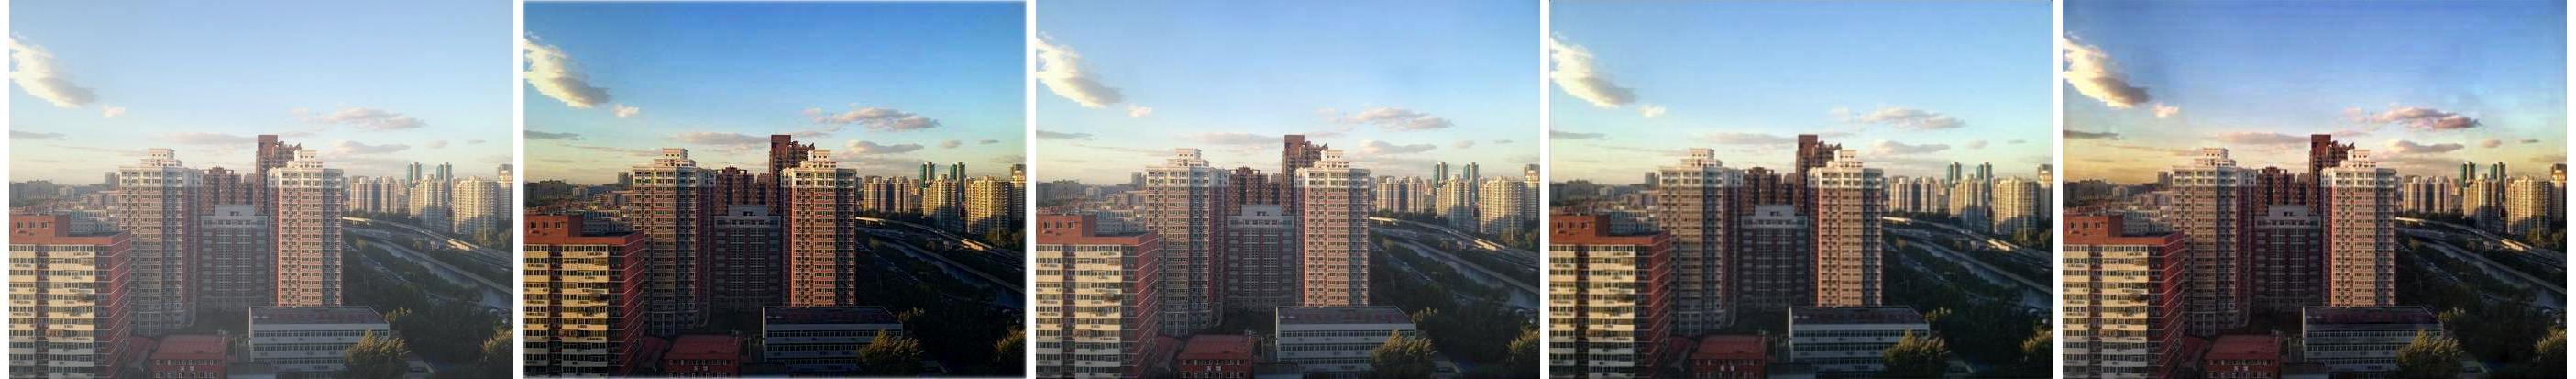
\includegraphics[width=16.5cm]{0_1.jpg} \\
    Hazy Image\qquad\quad\;\; AOD-Net\cite{li2017aod} \qquad GridDehazeNet\cite{liu2019griddehazenet} \;\, Wavelet-U-Net\cite{yang2019wavelet} \qquad GCA-Net\cite{chen2019gated}\\
    
    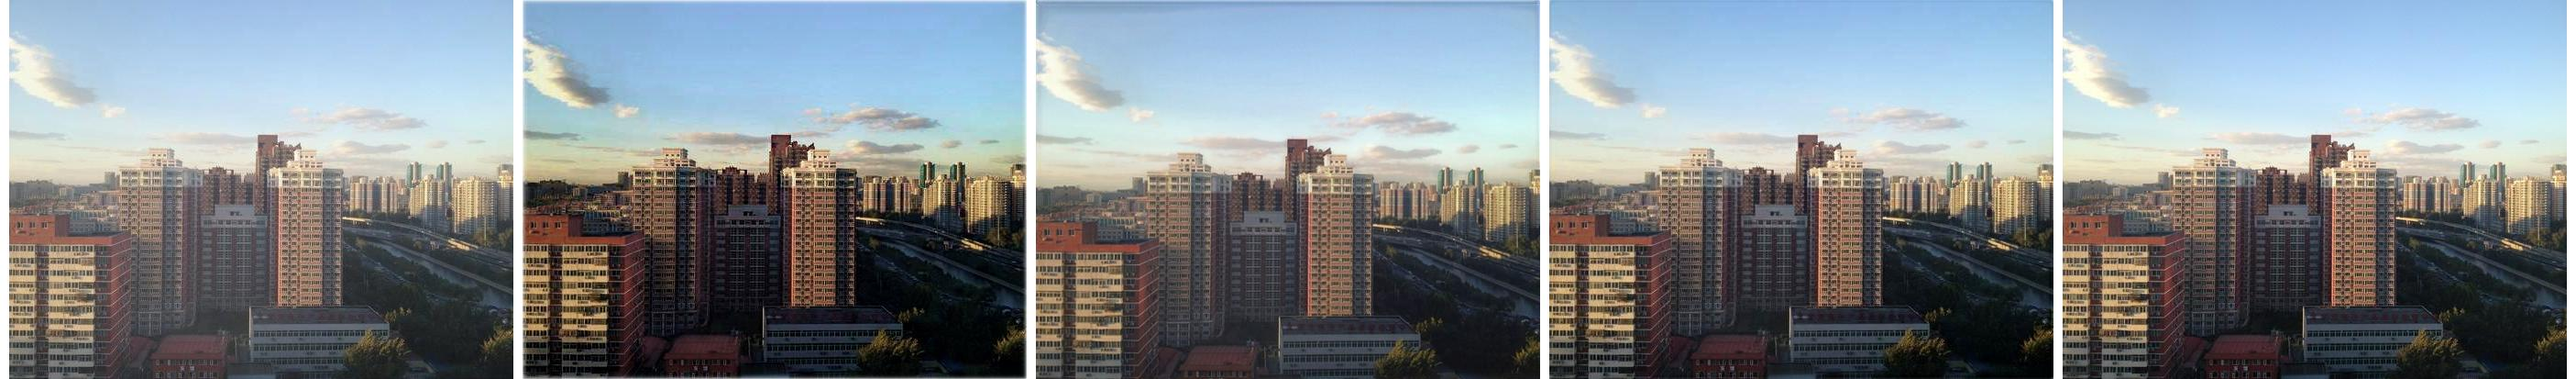
\includegraphics[width=16.5cm]{0_2.jpg} \\ 
    FFA-Net\cite{qin2020ffa} \qquad\quad\, LD-Net\cite{ullah2021light} \qquad\qquad\;\; D4\cite{yang2022d4} \qquad\qquad\; Ours (LFD-Net) \qquad\quad Ground Truth \\
    
    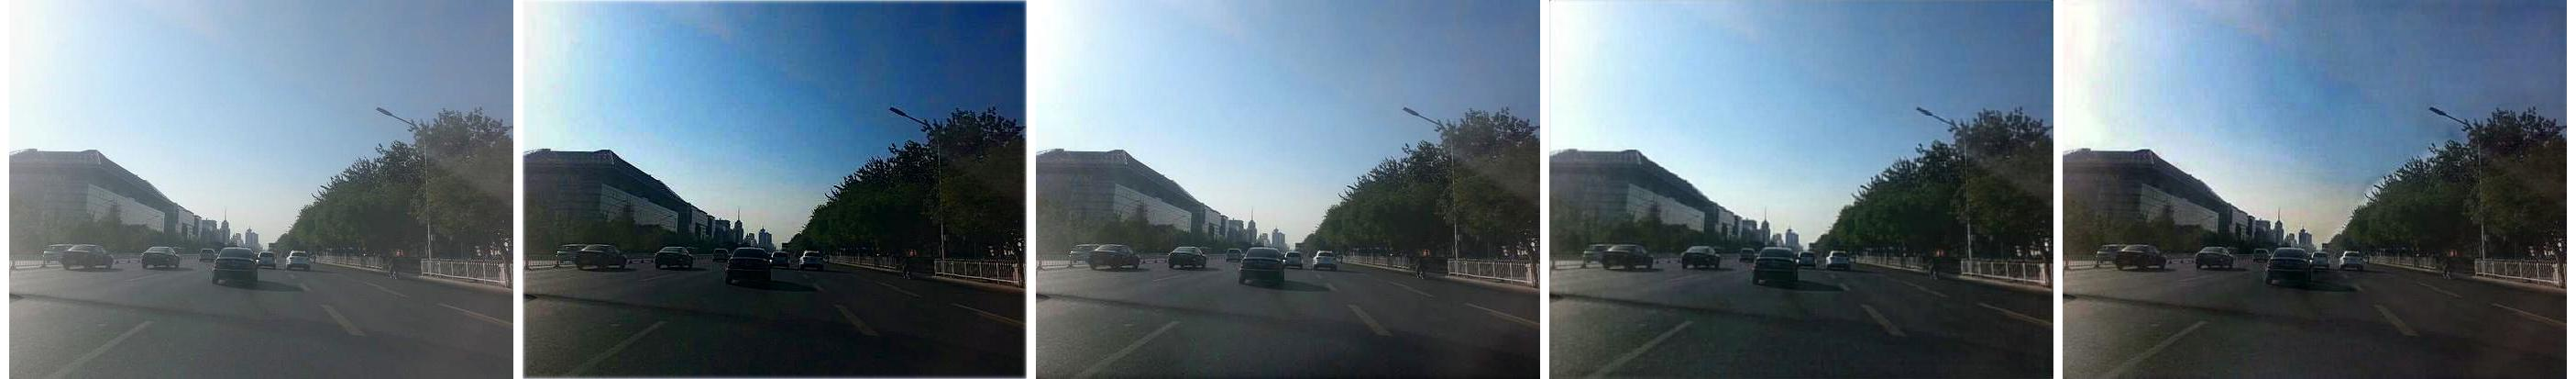
\includegraphics[width=16.5cm]{1_1.jpg} \\ 
    Hazy Image\qquad\quad\;\; AOD-Net\cite{li2017aod} \qquad GridDehazeNet\cite{liu2019griddehazenet} \;\, Wavelet-U-Net\cite{yang2019wavelet} \qquad GCA-Net\cite{chen2019gated}\\
    
    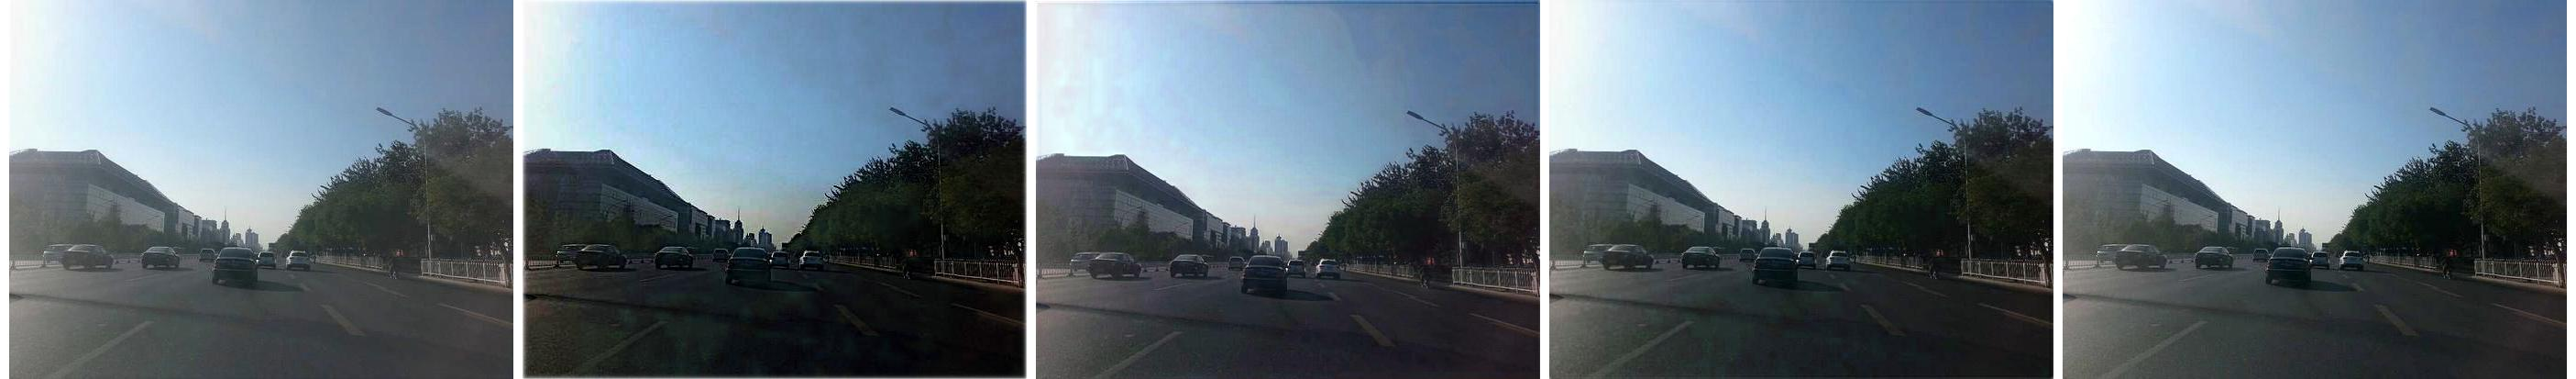
\includegraphics[width=16.5cm]{1_2.jpg} \\ 
    FFA-Net\cite{qin2020ffa} \qquad\quad\, LD-Net\cite{ullah2021light} \qquad\qquad\;\; D4\cite{yang2022d4} \qquad\qquad\; Ours (LFD-Net) \qquad\quad Ground Truth \\
    
    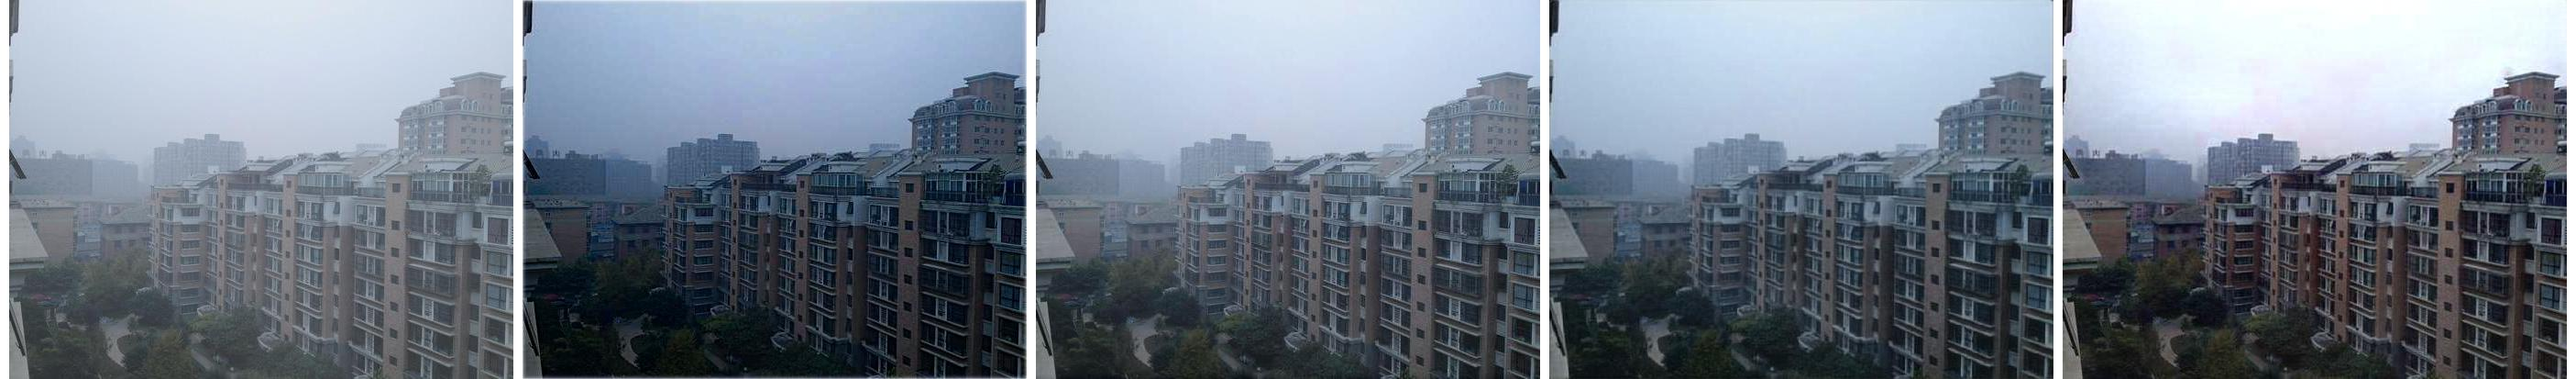
\includegraphics[width=16.5cm]{2_1.jpg} \\
    Hazy Image\qquad\quad\;\; AOD-Net\cite{li2017aod} \qquad GridDehazeNet\cite{liu2019griddehazenet} \;\, Wavelet-U-Net\cite{yang2019wavelet} \qquad GCA-Net\cite{chen2019gated}\\
    
    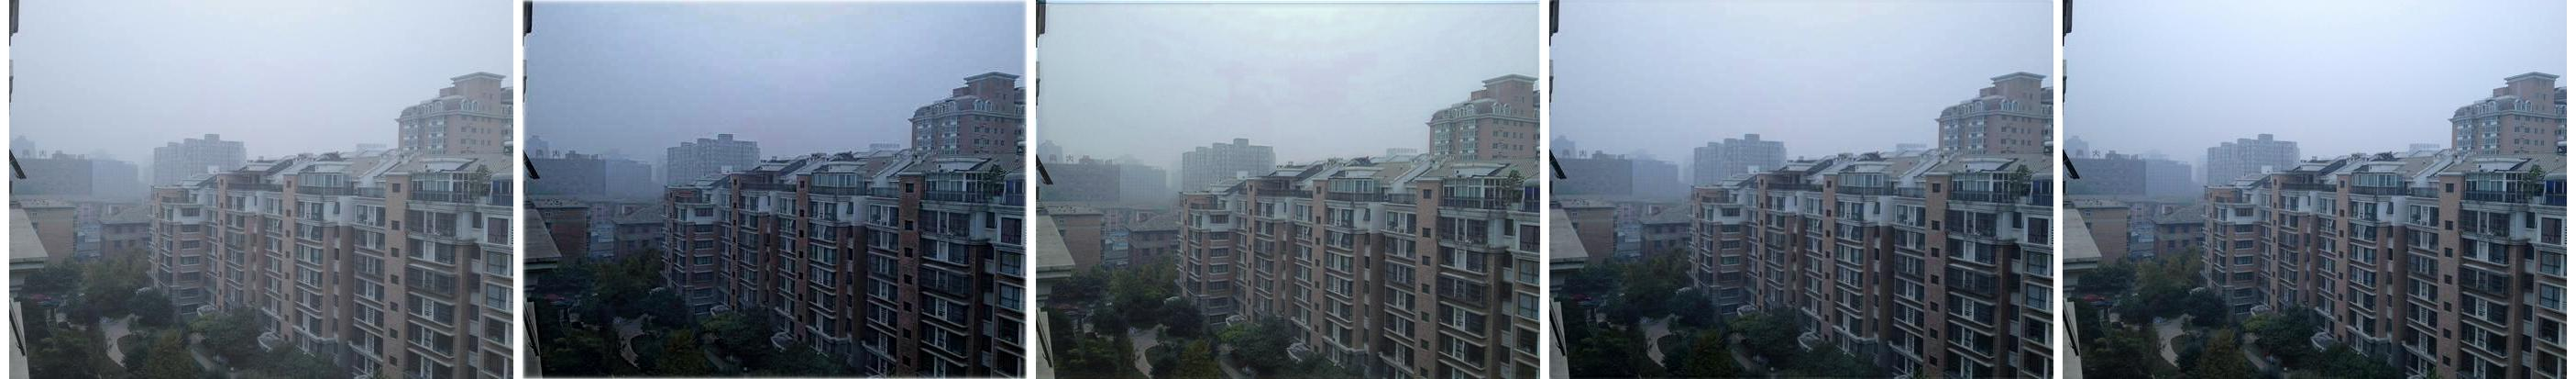
\includegraphics[width=16.5cm]{2_2.jpg} \\
    FFA-Net\cite{qin2020ffa} \qquad\quad\, LD-Net\cite{ullah2021light} \qquad\qquad\;\; D4\cite{yang2022d4} \qquad\qquad\; Ours (LFD-Net) \qquad\quad Ground Truth \\
    
    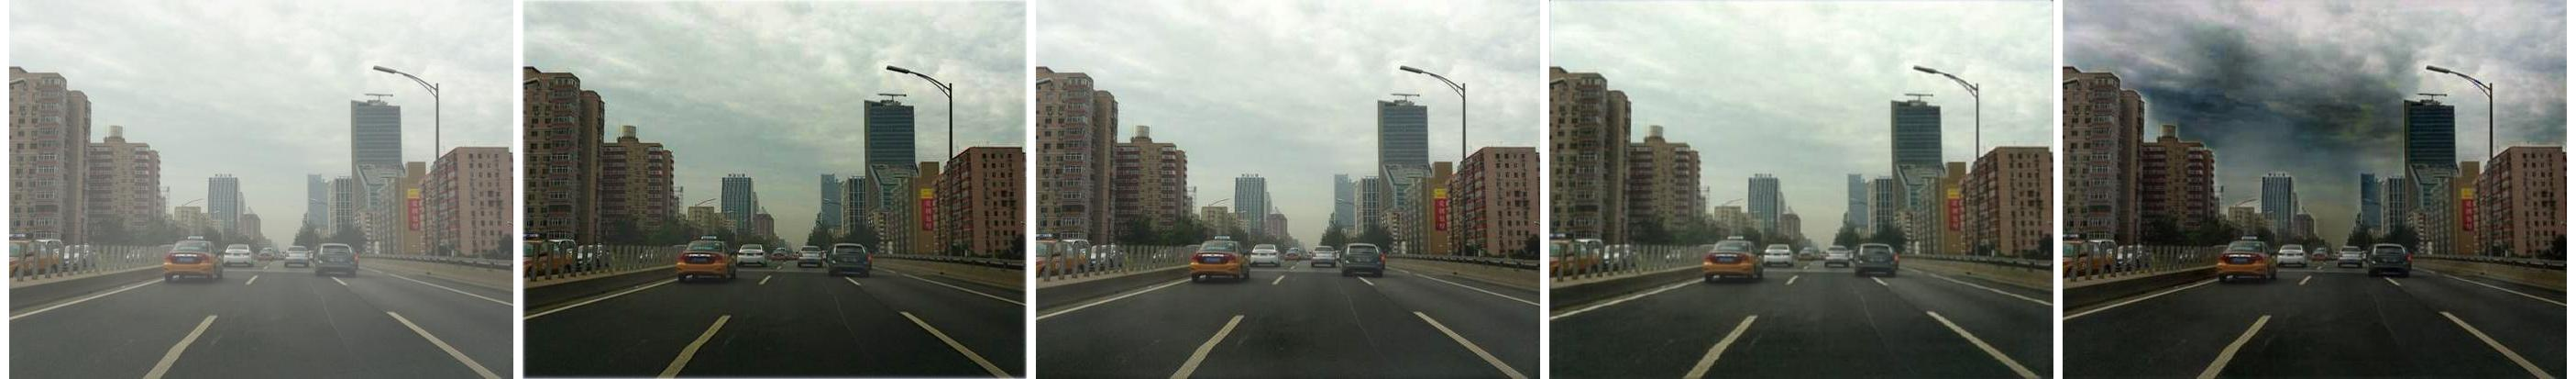
\includegraphics[width=16.5cm]{5_1.jpg} \\
    Hazy Image\qquad\quad\;\; AOD-Net\cite{li2017aod} \qquad GridDehazeNet\cite{liu2019griddehazenet} \;\, Wavelet-U-Net\cite{yang2019wavelet} \qquad GCA-Net\cite{chen2019gated}\\
    
    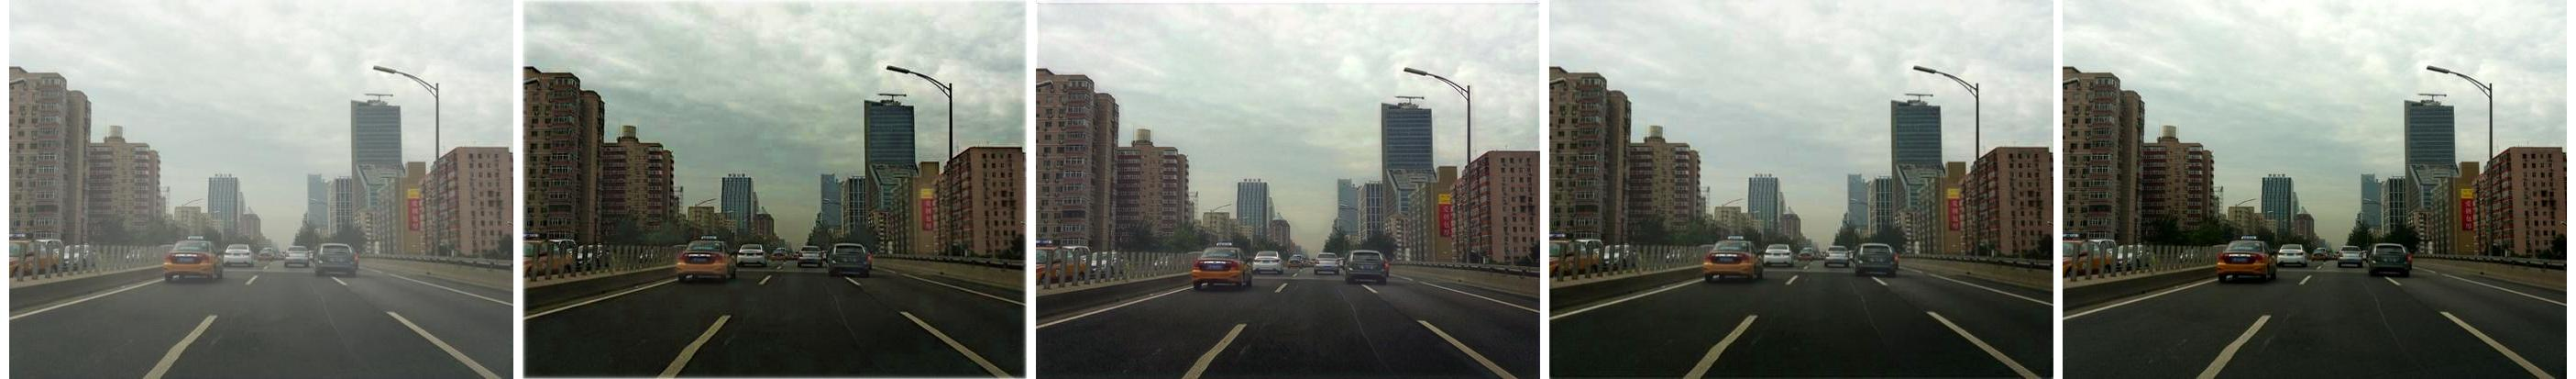
\includegraphics[width=16.5cm]{5_2.jpg} \\
    FFA-Net\cite{qin2020ffa} \qquad\quad\, LD-Net\cite{ullah2021light} \qquad\qquad\;\; D4\cite{yang2022d4} \qquad\qquad\; Ours (LFD-Net) \qquad\quad Ground Truth \\
    
    \caption{Visual Comparison on Outdoor SOTS. We compare our methods with AOD-Net\cite{li2017aod}, GridDehazeNet\cite{liu2019griddehazenet}, Wavelet-U-Net\cite{yang2019wavelet}, GCA-Net\cite{chen2019gated}, FFA-Net\cite{qin2020ffa}, LD-Net\cite{ullah2021light} and D4\cite{yang2022d4}. %AOD-Net and LD-Net produce relatively dark in visual quality. GCA-Net performs well on irregular haze but suffers from inconsistency in color blocks. Besides, 
    Our proposed method exhibits adaptability to diverse scenarios and possesses a noteworthy level of generalization.}
    \label{sots}
\end{figure*}

\begin{figure*}[ph!t]
    \centering
    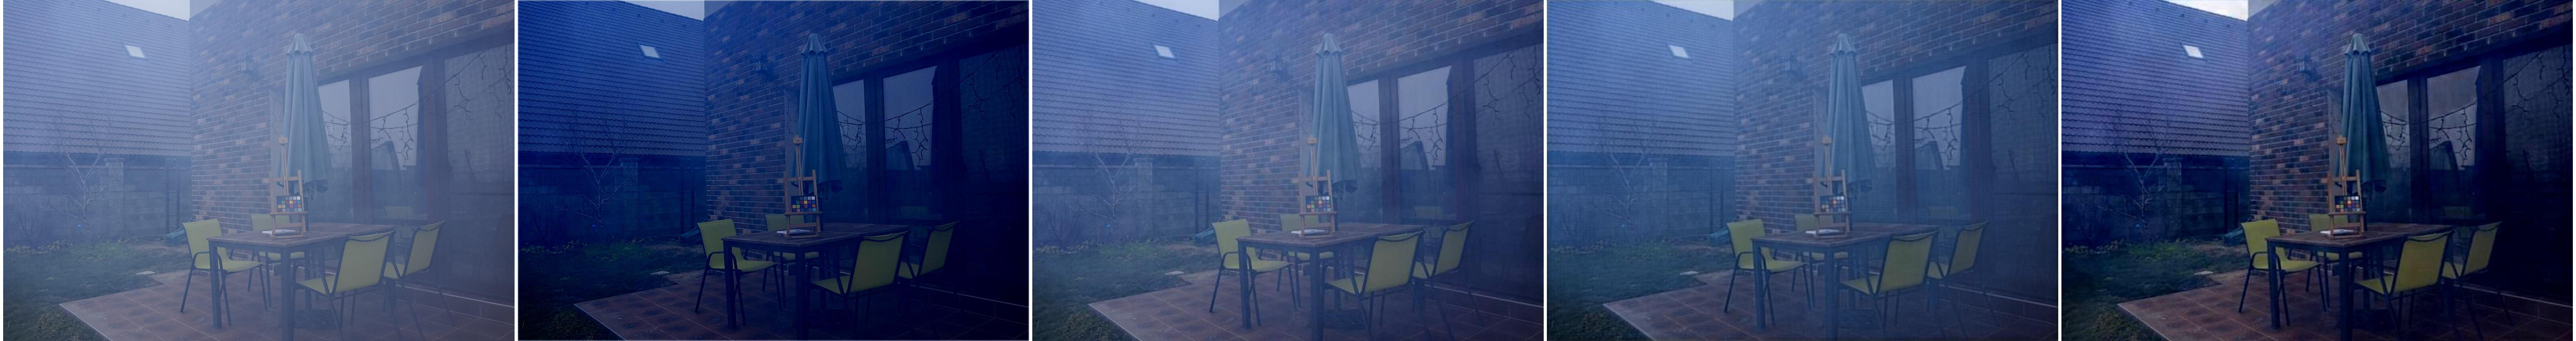
\includegraphics[width=16.5cm]{ohaze_0_1.jpg} \\
    Hazy Image\qquad\quad\;\; AOD-Net\cite{li2017aod} \qquad GridDehazeNet\cite{liu2019griddehazenet} \;\, Wavelet-U-Net\cite{yang2019wavelet} \qquad GCA-Net\cite{chen2019gated}\\
    
    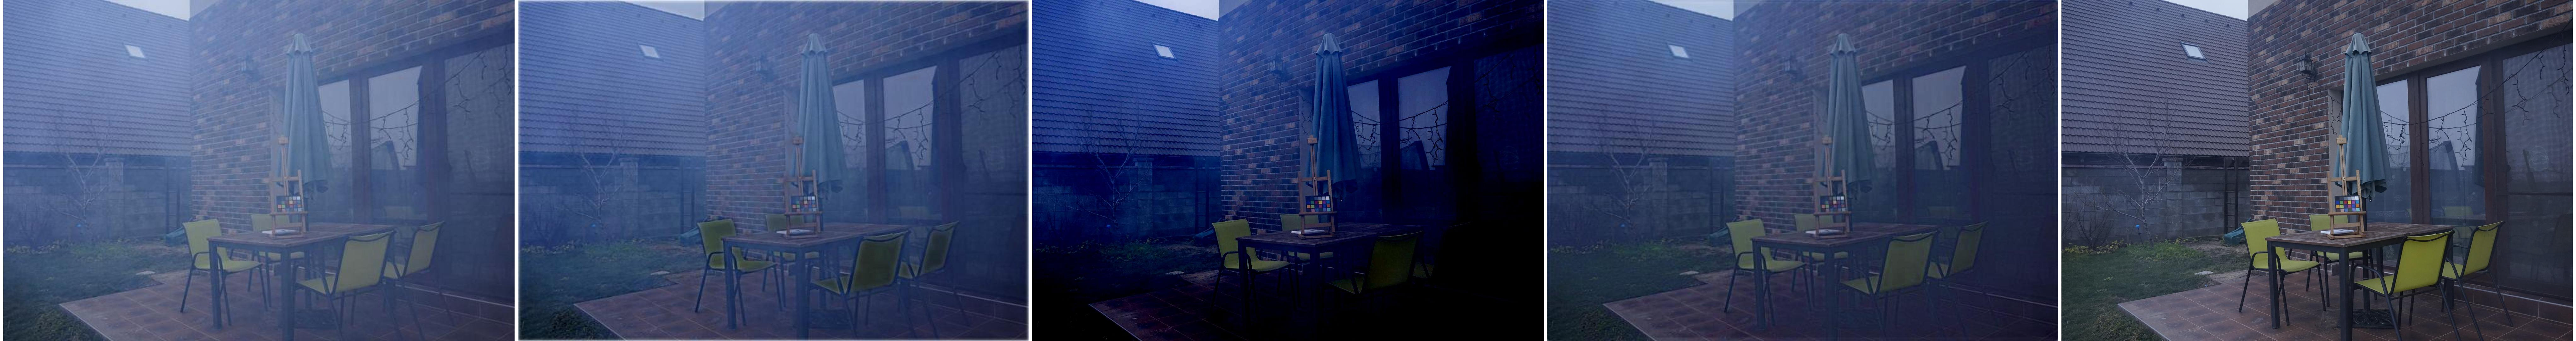
\includegraphics[width=16.5cm]{ohaze_0_2.jpg} \\ 
    FFA-Net\cite{qin2020ffa} \qquad\quad\, LD-Net\cite{ullah2021light} \qquad\qquad\;\; D4\cite{yang2022d4} \qquad\qquad\; Ours (LFD-Net) \qquad\quad Ground Truth \\
    
    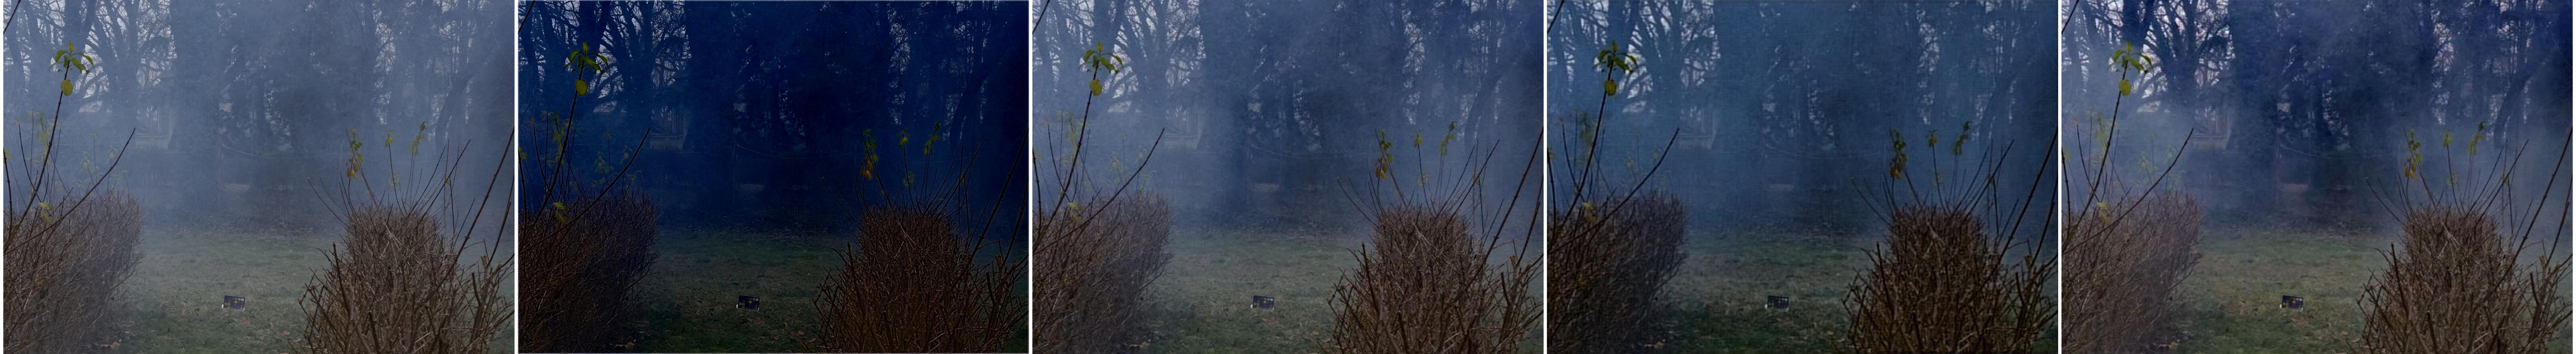
\includegraphics[width=16.5cm]{ohaze_1_1.jpg} \\ 
    Hazy Image\qquad\quad\;\; AOD-Net\cite{li2017aod} \qquad GridDehazeNet\cite{liu2019griddehazenet} \;\, Wavelet-U-Net\cite{yang2019wavelet} \qquad GCA-Net\cite{chen2019gated}\\
    
    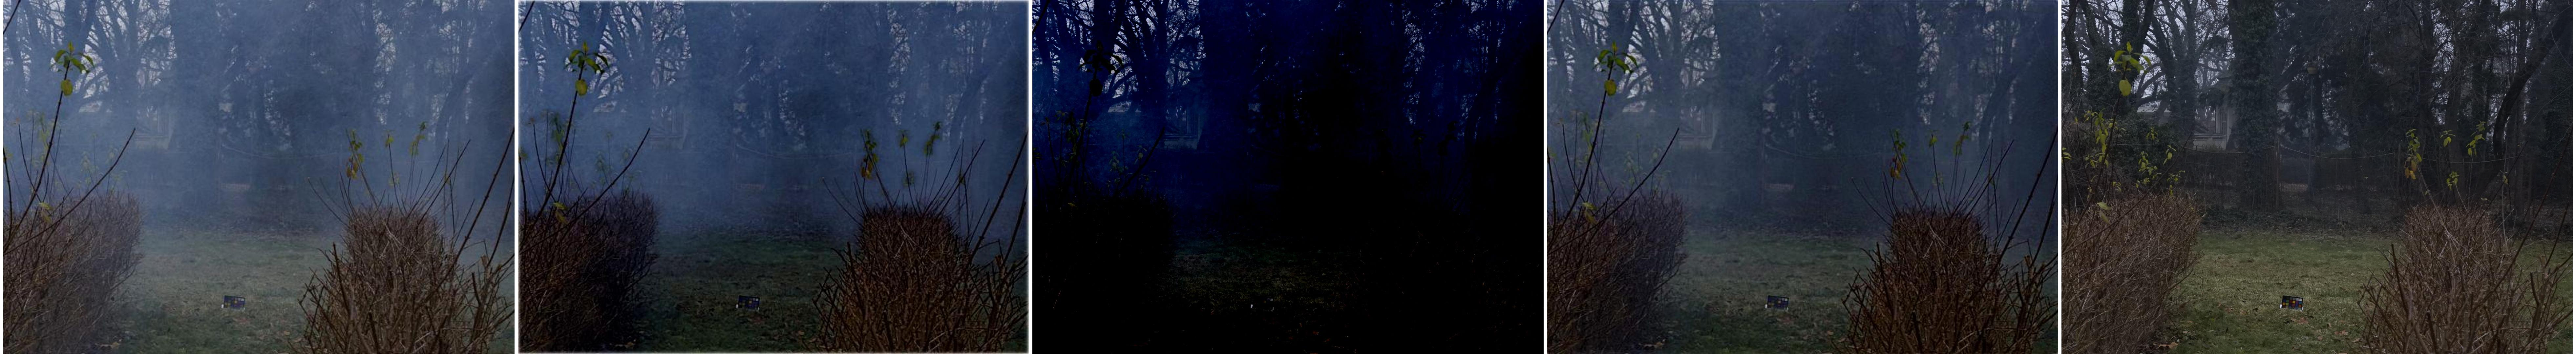
\includegraphics[width=16.5cm]{ohaze_1_2.jpg} \\ 
    FFA-Net\cite{qin2020ffa} \qquad\quad\, LD-Net\cite{ullah2021light} \qquad\qquad\;\; D4\cite{yang2022d4} \qquad\qquad\; Ours (LFD-Net) \qquad\quad Ground Truth \\
    
    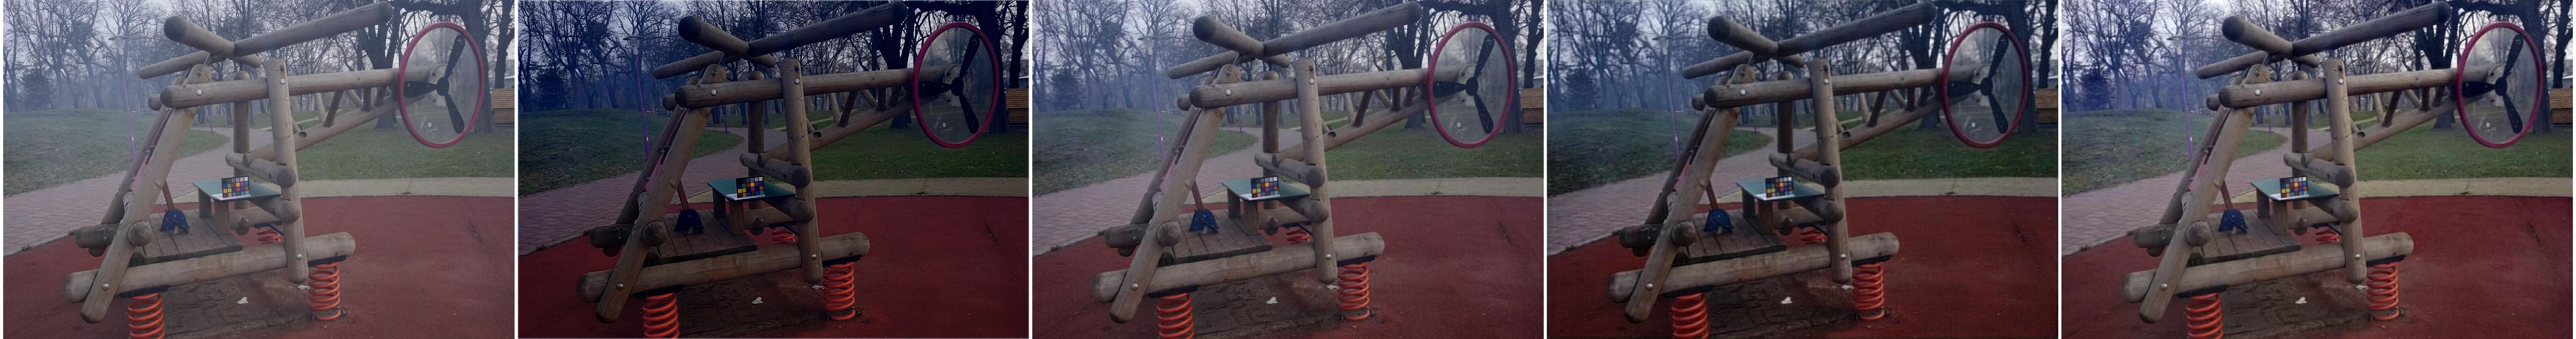
\includegraphics[width=16.5cm]{ohaze_2_1.jpg} \\
    Hazy Image\qquad\quad\;\; AOD-Net\cite{li2017aod} \qquad GridDehazeNet\cite{liu2019griddehazenet} \;\, Wavelet-U-Net\cite{yang2019wavelet} \qquad GCA-Net\cite{chen2019gated}\\
    
    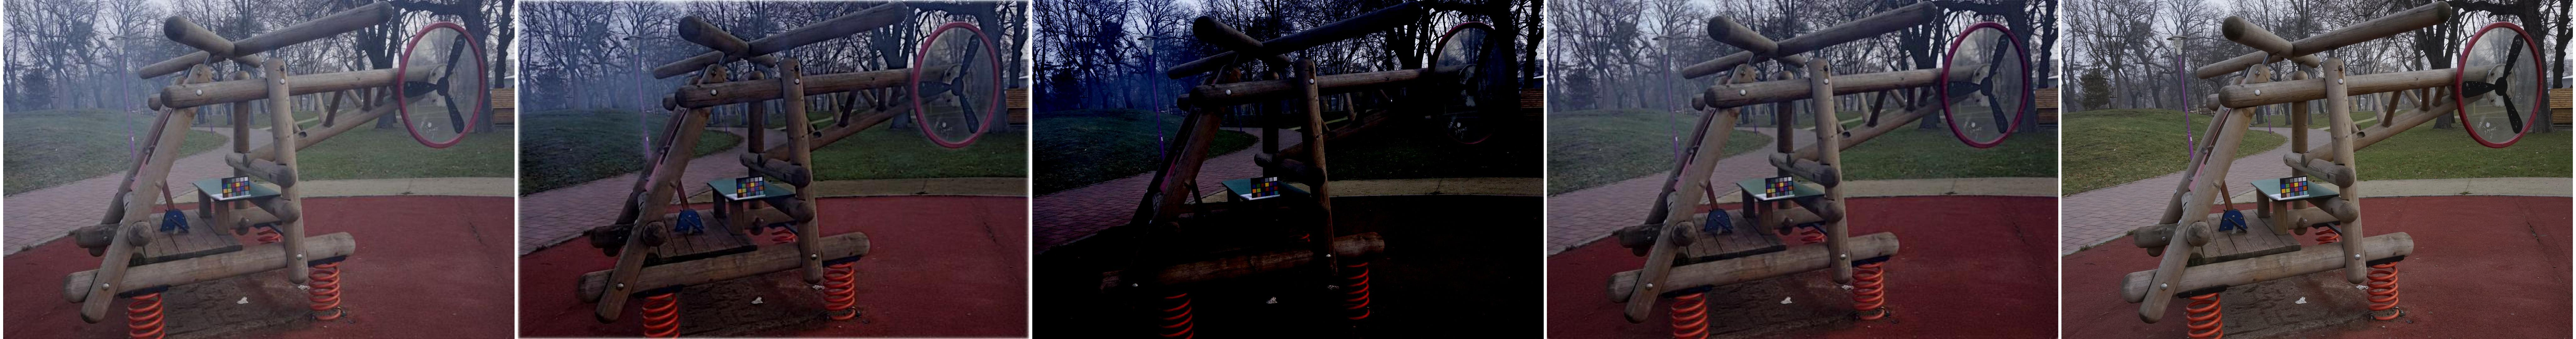
\includegraphics[width=16.5cm]{ohaze_2_2.jpg} \\
    FFA-Net\cite{qin2020ffa} \qquad\quad\, LD-Net\cite{ullah2021light} \qquad\qquad\;\; D4\cite{yang2022d4} \qquad\qquad\; Ours (LFD-Net) \qquad\quad Ground Truth \\
    
    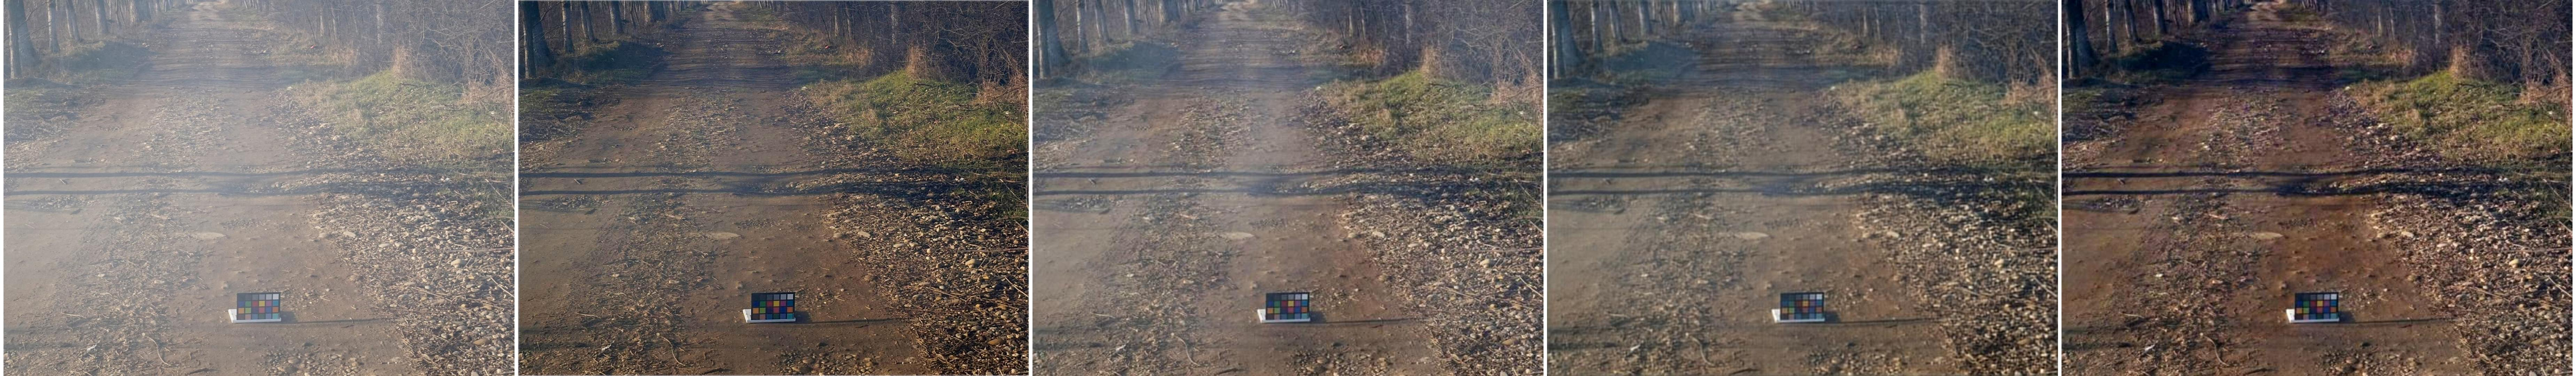
\includegraphics[width=16.5cm]{ohaze_3_1.jpg} \\
    Hazy Image\qquad\quad\;\; AOD-Net\cite{li2017aod} \qquad GridDehazeNet\cite{liu2019griddehazenet} \;\, Wavelet-U-Net\cite{yang2019wavelet} \qquad GCA-Net\cite{chen2019gated}\\
    
    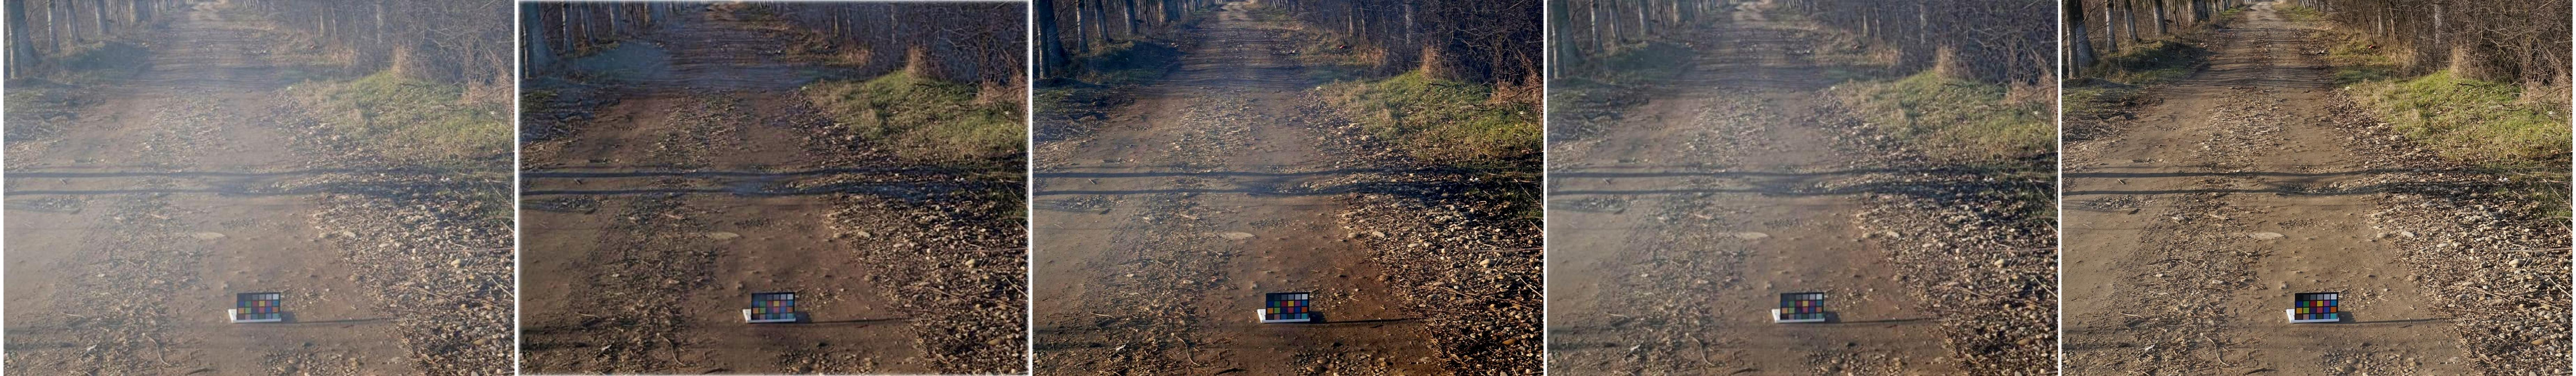
\includegraphics[width=16.5cm]{ohaze_3_2.jpg} \\
    FFA-Net\cite{qin2020ffa} \qquad\quad\, LD-Net\cite{ullah2021light} \qquad\qquad\;\; D4\cite{yang2022d4} \qquad\qquad\; Ours (LFD-Net) \qquad\quad Ground Truth \\
    
    \caption{Visual Comparison Results on O-HAZE. We compare our methods with AOD-Net\cite{li2017aod}, GridDehazeNet\cite{liu2019griddehazenet}, Wavelet-U-Net\cite{yang2019wavelet}, GCA-Net\cite{chen2019gated}, FFA-Net\cite{qin2020ffa}, LD-Net\cite{ullah2021light} and D4\cite{yang2022d4}. AOD-Net and LD-Net produce relatively dark in visual quality. GCA-Net performs well on irregular haze but suffers from inconsistency in color blocks. Our proposed method exhibits adaptability to diverse scenarios and possesses a noteworthy level of generalization. }
    \label{ohaze}
\end{figure*}

\begin{figure*}[pht]
    \centering
    %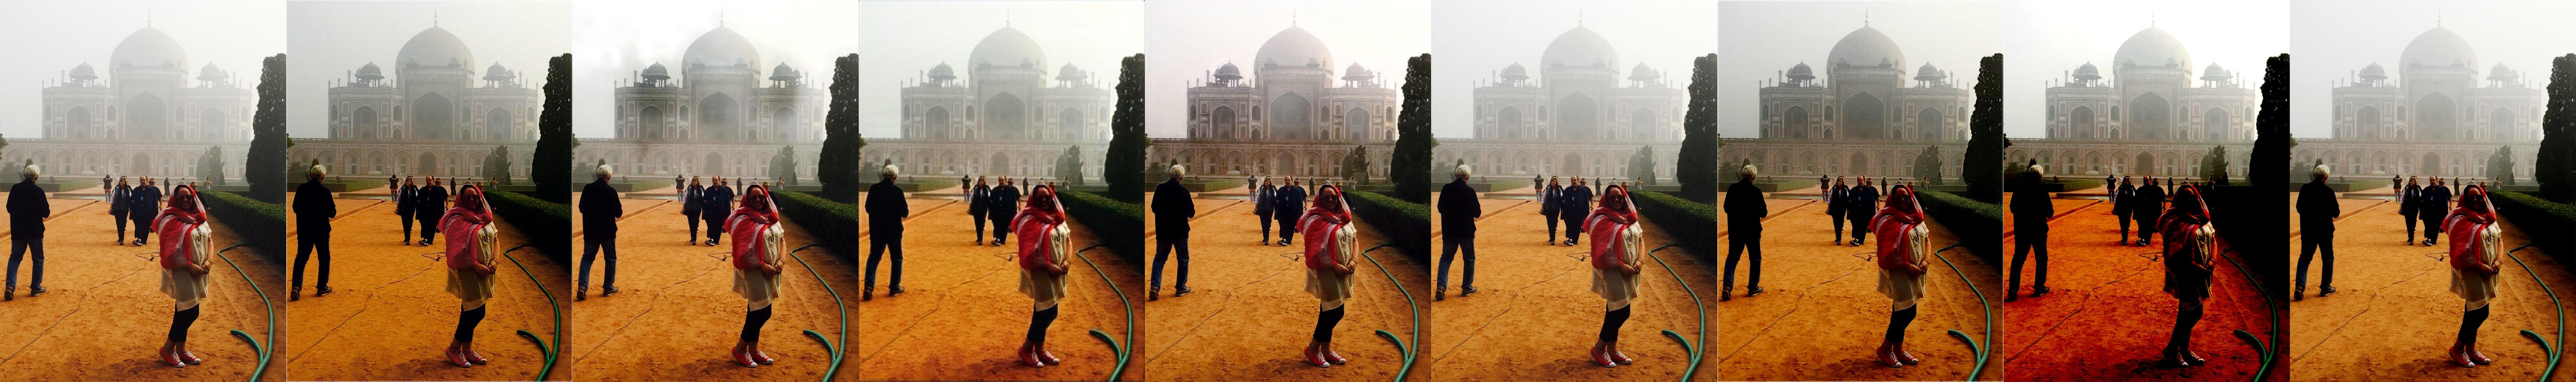
\includegraphics[width=\textwidth]{hsts_1.jpg}
    
\includegraphics[width=\textwidth]{hsts_2.jpg}
    
\includegraphics[width=\textwidth]{hsts_3.jpg}
    
\includegraphics[width=\textwidth]{hsts_4.jpg}
    %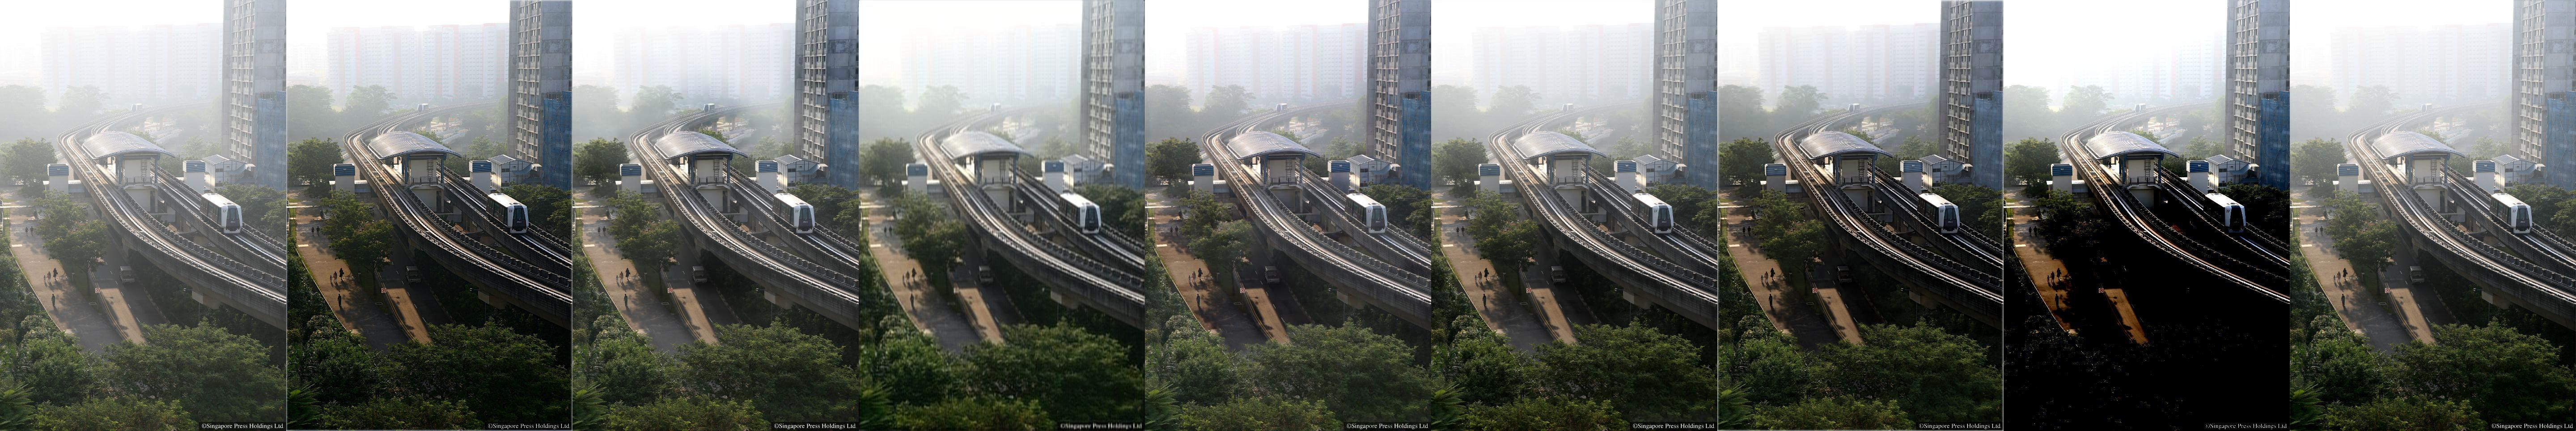
\includegraphics[width=\textwidth]{hsts_5.jpg}
    
\includegraphics[width=\textwidth]{hsts_6.jpg}
    
\includegraphics[width=\textwidth]{hsts_7.jpg}
    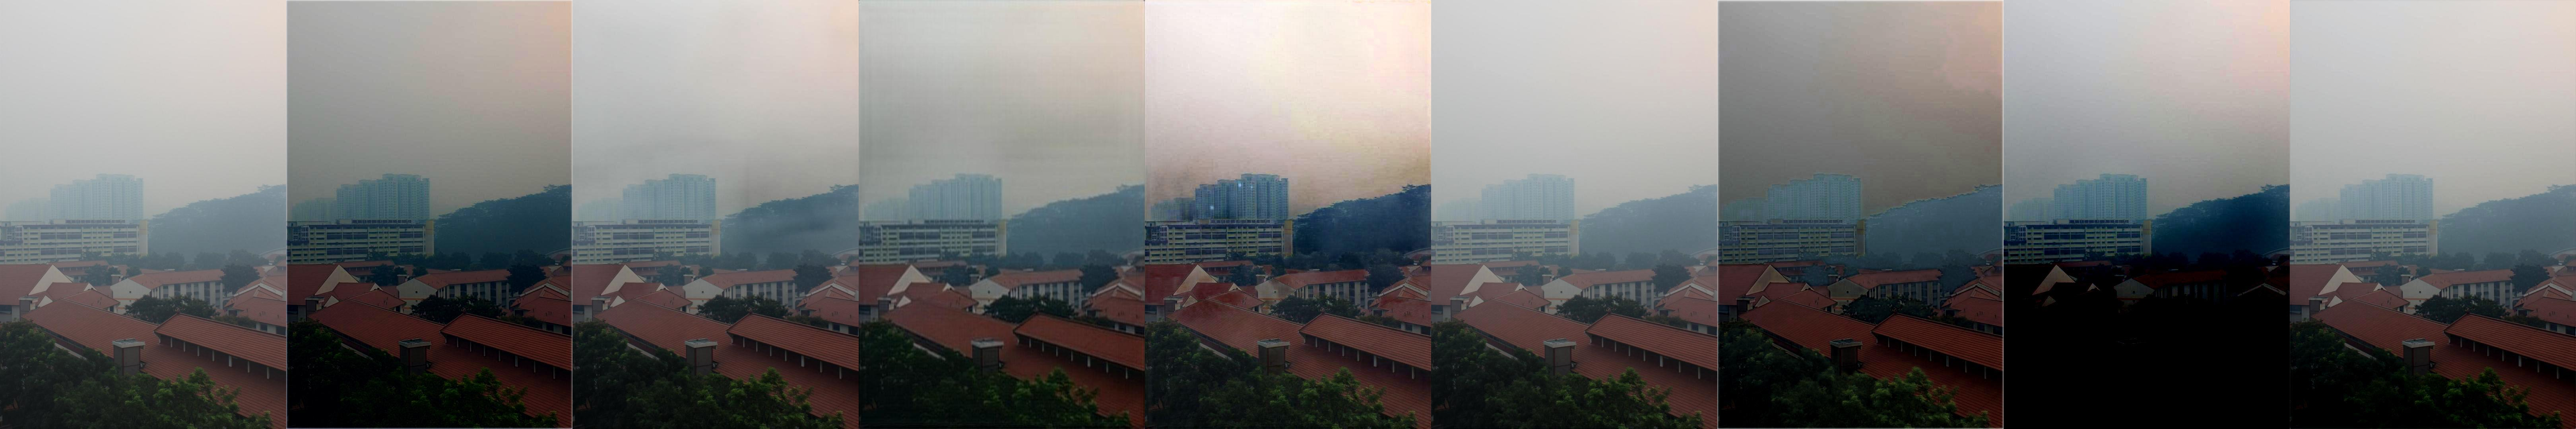
\includegraphics[width=\textwidth]{hsts_8.jpg}
    
\includegraphics[width=\textwidth]{hsts_9.jpg}
    %
\includegraphics[width=\textwidth]{hsts_10.jpg}
    (a) \qquad\quad\;\;\;\ (b) \qquad\quad\;\;\;\ (c) \qquad\quad\;\;\;\ (d) \qquad\quad\;\;\;\, (e) \qquad\quad\;\;\;\, (f) \qquad\quad\;\;\;\ (g) \qquad\quad\;\;\;\ (h) \qquad\quad\;\;\;\ (i)
    \caption{Visual Comparison Results on Real-world HSTS. (a) Hazy image, (b) AOD-Net\cite{li2017aod}, (c) GridDehazeNet\cite{liu2019griddehazenet}, (d) Wavelet-U-Net\cite{yang2019wavelet}, (e) GCA-Net\cite{chen2019gated}, (f) FFA-Net\cite{qin2020ffa}, (g) LD-Net\cite{ullah2021light}, (h) D4\cite{yang2022d4} and (i) Ours (LFD-Net). Our proposed method exhibits adaptability to diverse scenarios and possesses a noteworthy level of generalization.}
    \label{hsts}
\end{figure*}

\begin{figure*}[pht]
    \centering
    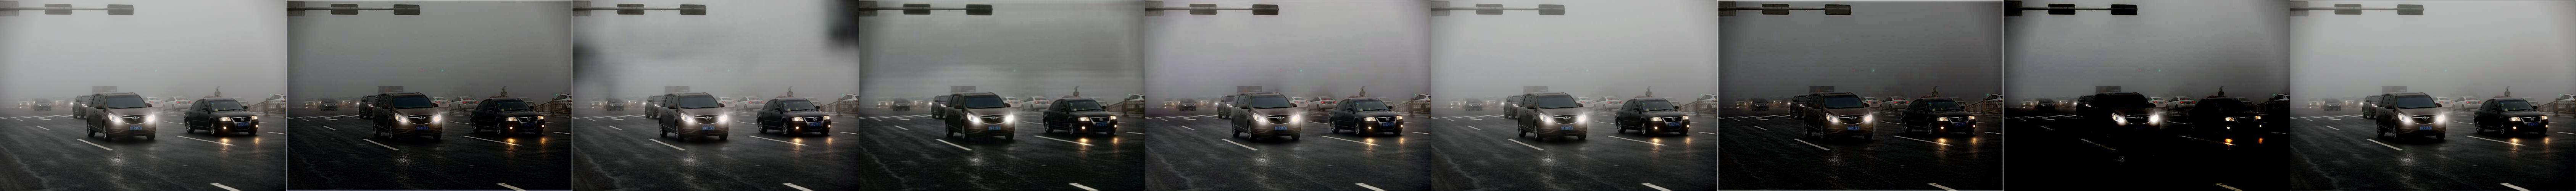
\includegraphics[width=\textwidth]{own_6.jpg}
    
\includegraphics[width=\textwidth]{own_8.jpg}
    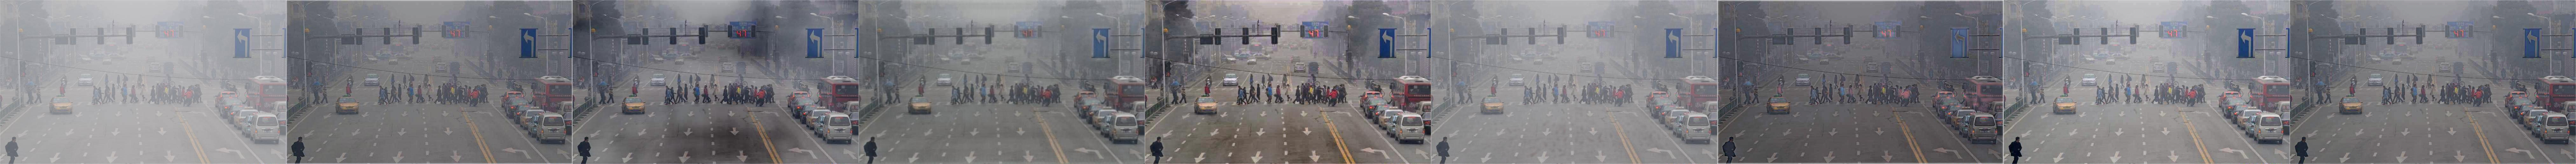
\includegraphics[width=\textwidth]{own_14.jpg}
    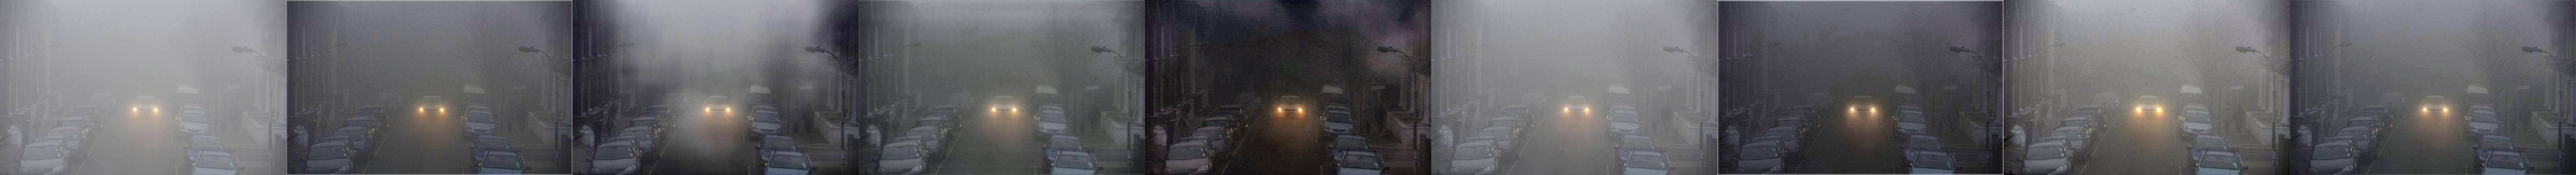
\includegraphics[width=\textwidth]{own_16.jpg}
    
\includegraphics[width=\textwidth]{own_19.jpg}
    
\includegraphics[width=\textwidth]{own_24.jpg}
    
\includegraphics[width=\textwidth]{own_26.jpg}
    %
\includegraphics[width=\textwidth]{own_27.jpg}
    (a) \qquad\quad\;\;\;\ (b) \qquad\quad\;\;\;\ (c) \qquad\quad\;\;\;\ (d) \qquad\quad\;\;\;\, (e) \qquad\quad\;\;\;\, (f) \qquad\quad\;\;\;\ (g) \qquad\quad\;\;\;\ (h) \qquad\quad\;\;\;\ (i)
    \caption{Visual Comparison Results on Randomly Selected Real-world Images. (a) Hazy image, (b) AOD-Net\cite{li2017aod}, (c) GridDehazeNet\cite{liu2019griddehazenet}, (d) Wavelet-U-Net\cite{yang2019wavelet}, (e) GCA-Net\cite{chen2019gated}, (f) FFA-Net\cite{qin2020ffa}, (g) LD-Net\cite{ullah2021light}, (h) D4\cite{yang2022d4} and (i) Ours (LFD-Net). Our proposed method exhibits adaptability to diverse scenarios and possesses a noteworthy level of generalization.}
    \label{own}
\end{figure*}

\begin{figure*}[pht]
    \centering
    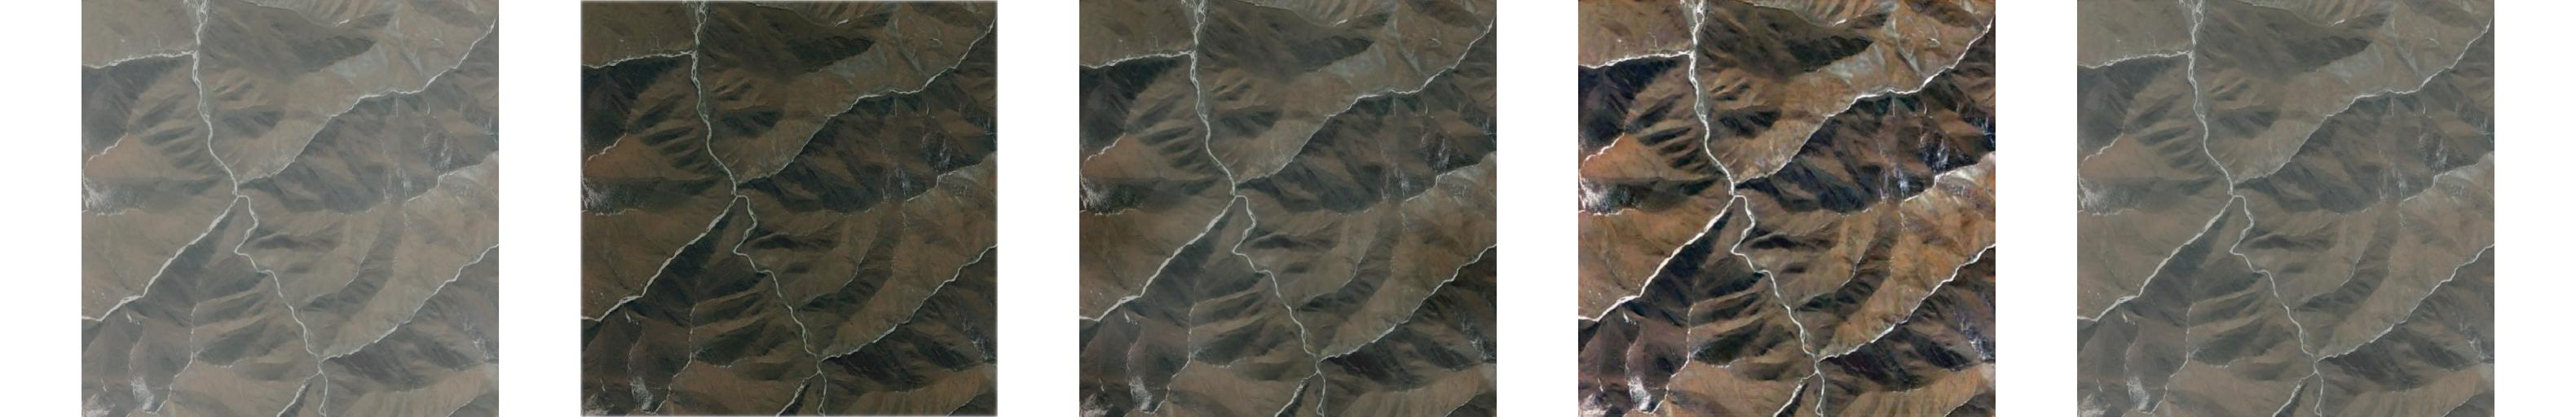
\includegraphics[width=14.5cm]{rice_0_1.jpg} \\
    Hazy Image\qquad\;\ AOD-Net\cite{li2017aod} \;\ GridDehazeNet\cite{liu2019griddehazenet} \;\; GCA-Net\cite{chen2019gated} \quad\; FFA-Net\cite{qin2020ffa}\\
    
    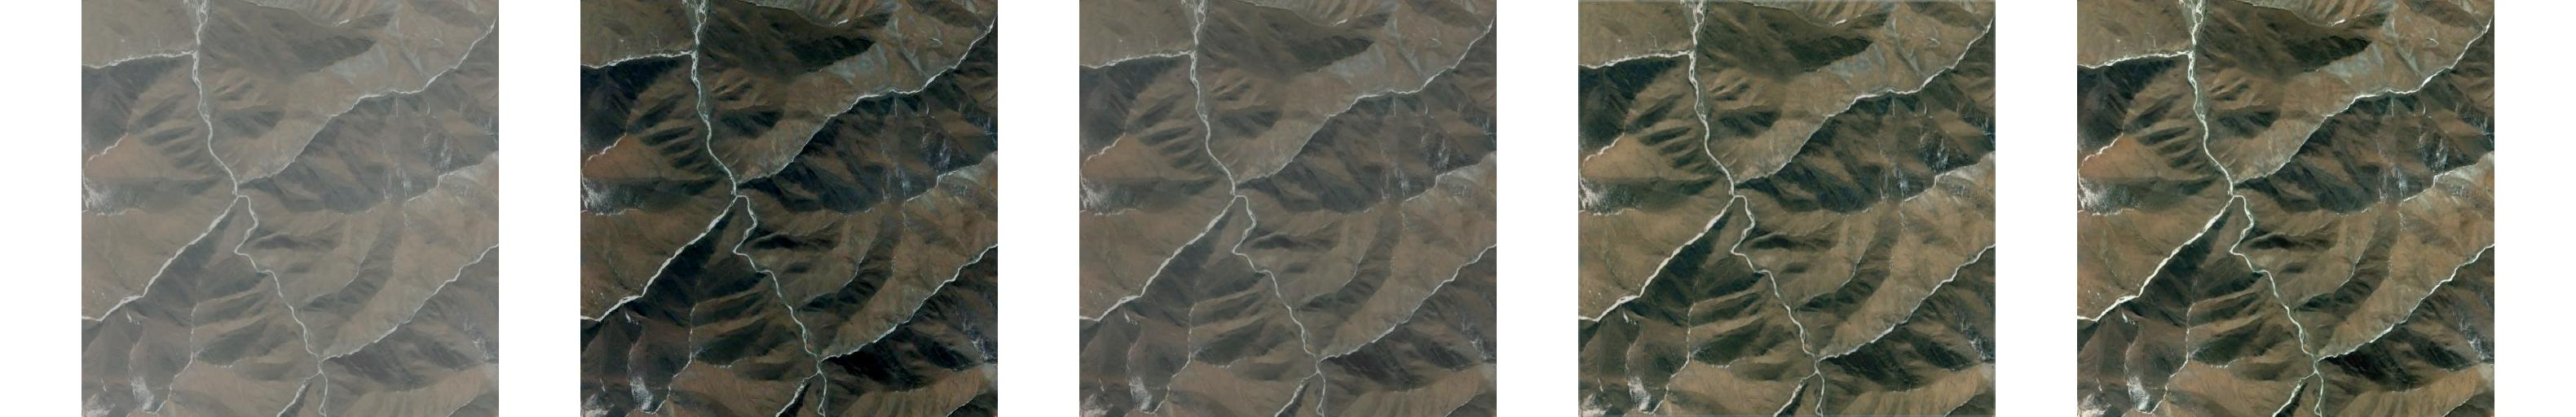
\includegraphics[width=14.5cm]{rice_0_2.jpg} \\ 
    MSBDN \cite{msbdn2020}\quad\quad\quad\, D4\cite{yang2022d4} \quad\quad DehazeFormer\cite{dehazeformer} \;\, Ours (LFD-Net) \quad\, Ground Truth \\
    
    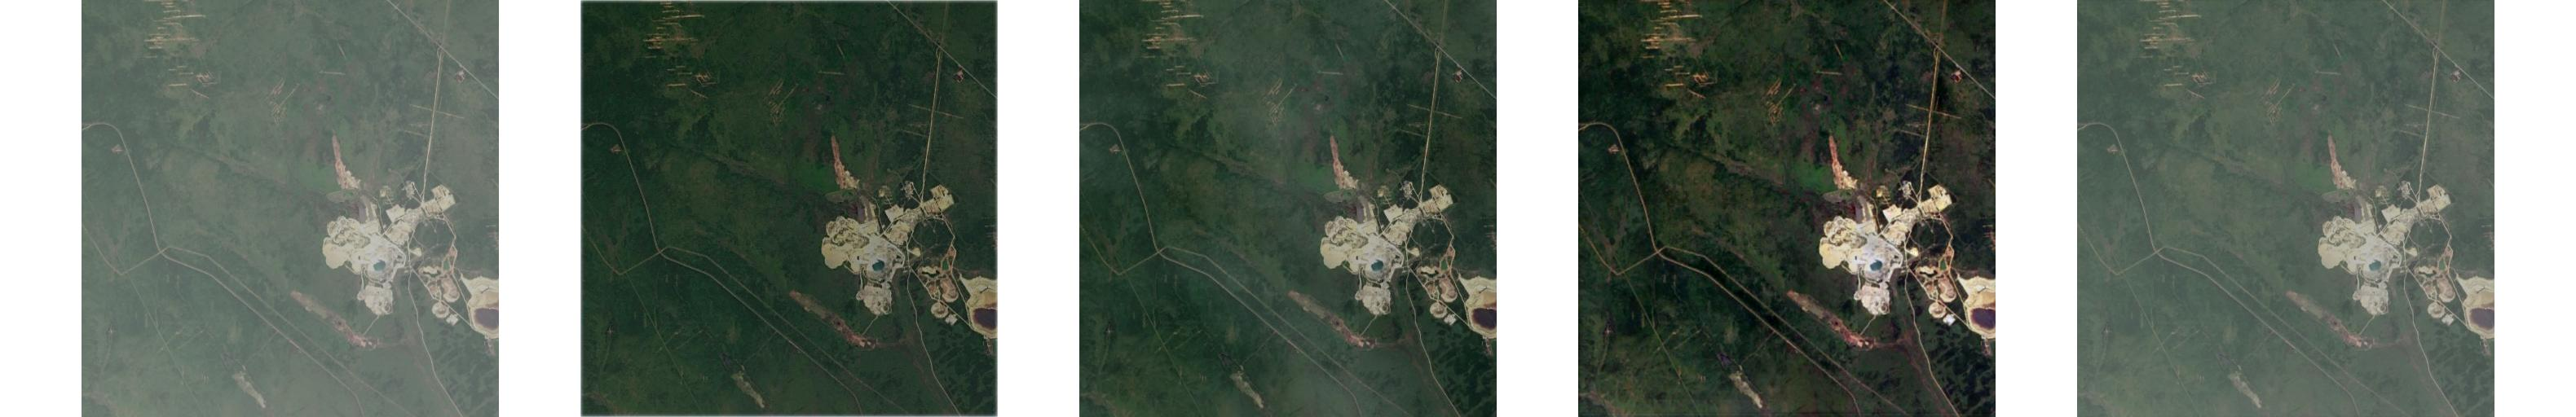
\includegraphics[width=14.5cm]{rice_1_1.jpg} \\ 
    Hazy Image\qquad\;\ AOD-Net\cite{li2017aod} \;\ GridDehazeNet\cite{liu2019griddehazenet} \;\; GCA-Net\cite{chen2019gated} \quad\; FFA-Net\cite{qin2020ffa}\\
    
    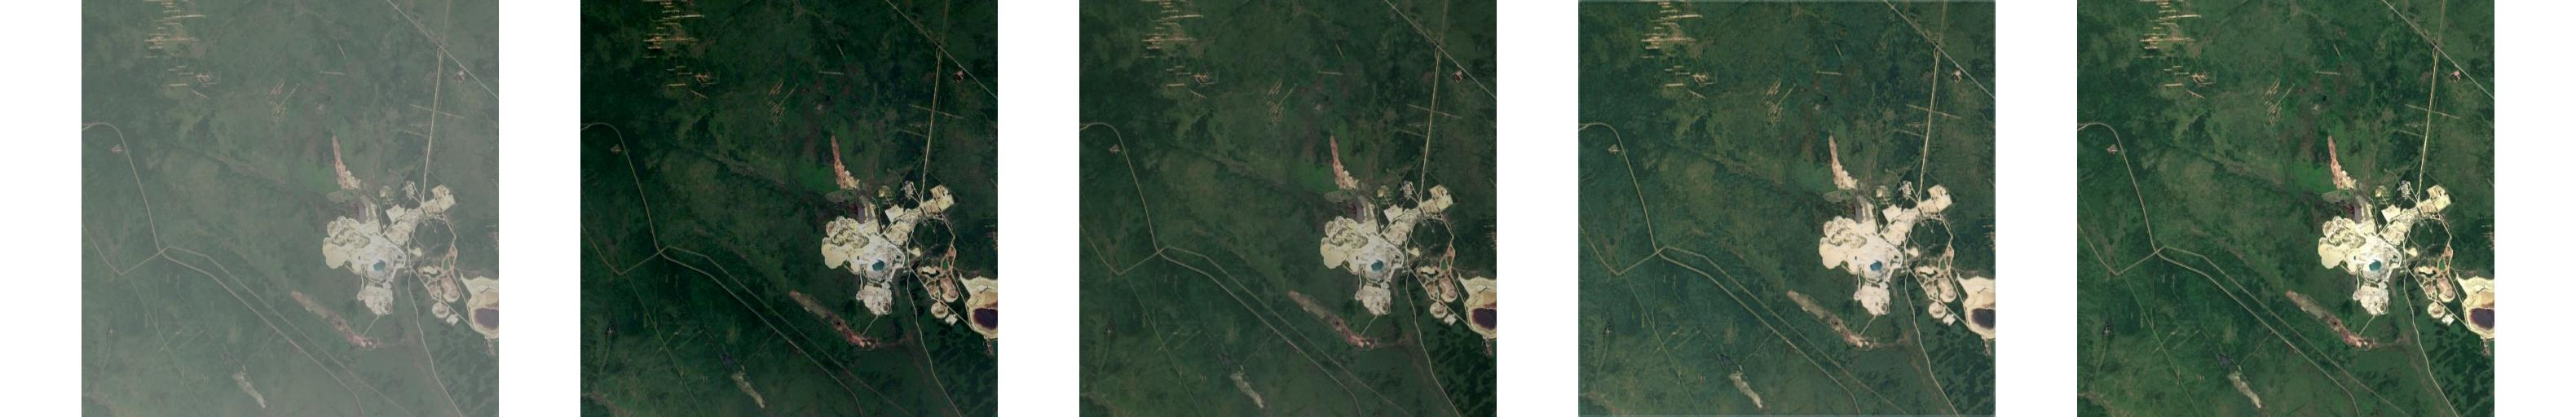
\includegraphics[width=14.5cm]{rice_1_2.jpg} \\ 
    MSBDN \cite{msbdn2020}\quad\quad\quad\, D4\cite{yang2022d4} \quad\quad DehazeFormer\cite{dehazeformer} \;\, Ours (LFD-Net) \quad\, Ground Truth \\
    
    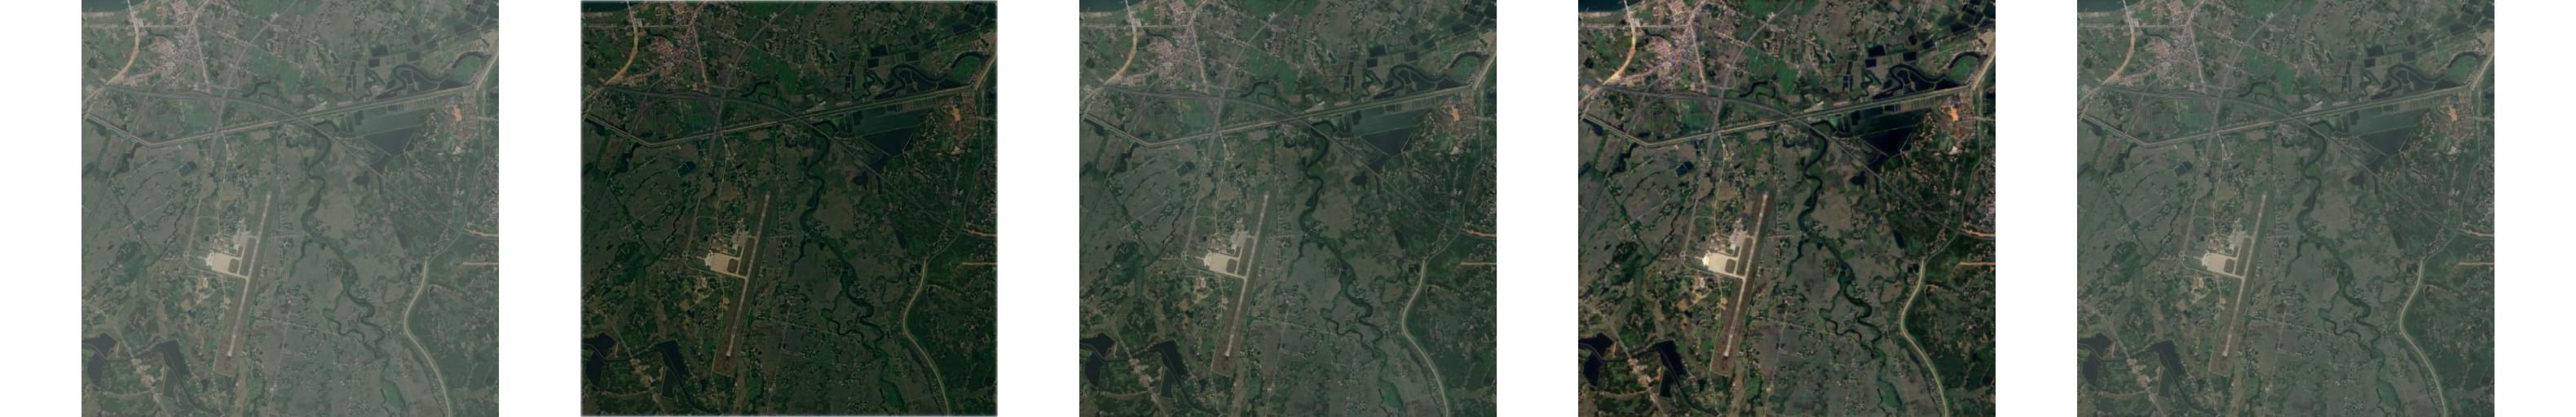
\includegraphics[width=14.5cm]{rice_2_1.jpg} \\
    Hazy Image\qquad\;\ AOD-Net\cite{li2017aod} \;\ GridDehazeNet\cite{liu2019griddehazenet} \;\; GCA-Net\cite{chen2019gated} \quad\; FFA-Net\cite{qin2020ffa}\\   
    
    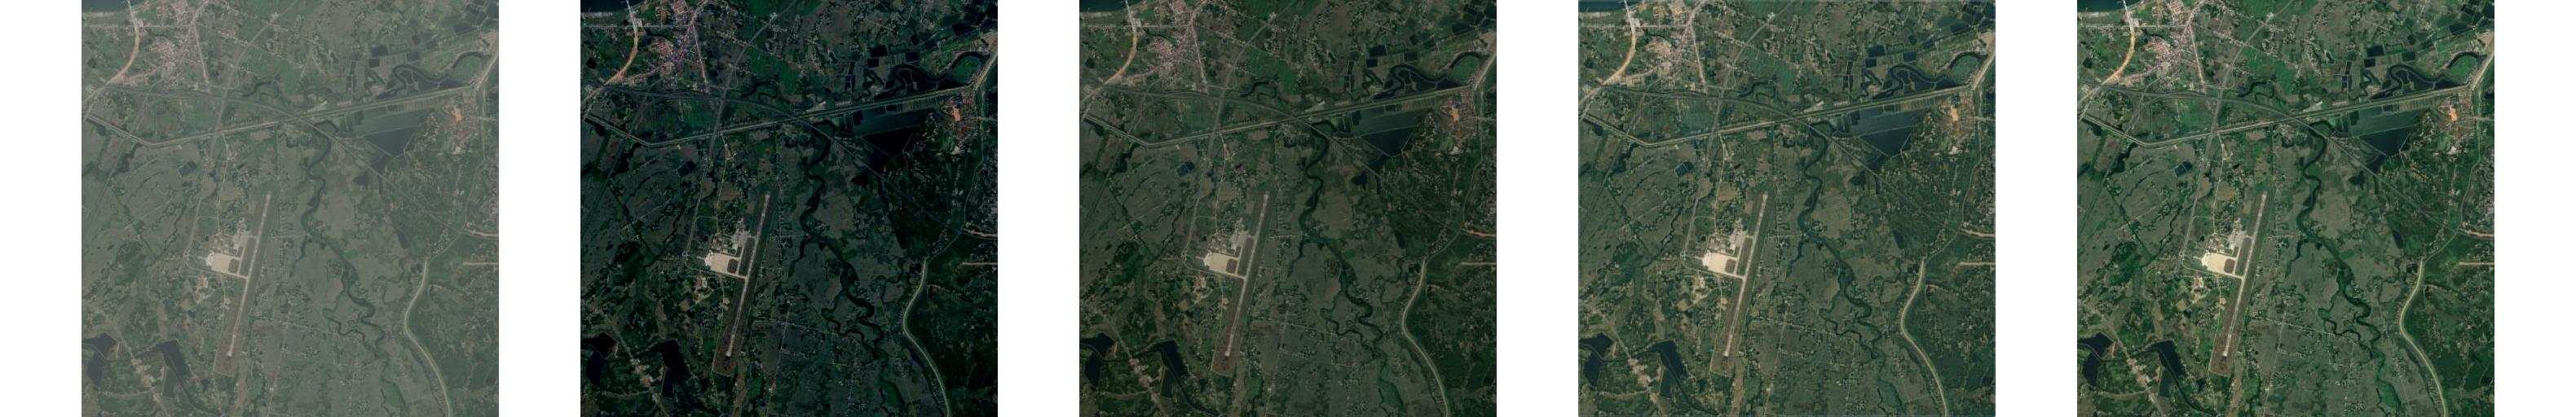
\includegraphics[width=14.5cm]{rice_2_2.jpg} \\
    MSBDN \cite{msbdn2020}\quad\quad\quad\, D4\cite{yang2022d4} \quad\quad DehazeFormer\cite{dehazeformer} \;\, Ours (LFD-Net) \quad\, Ground Truth \\
    
    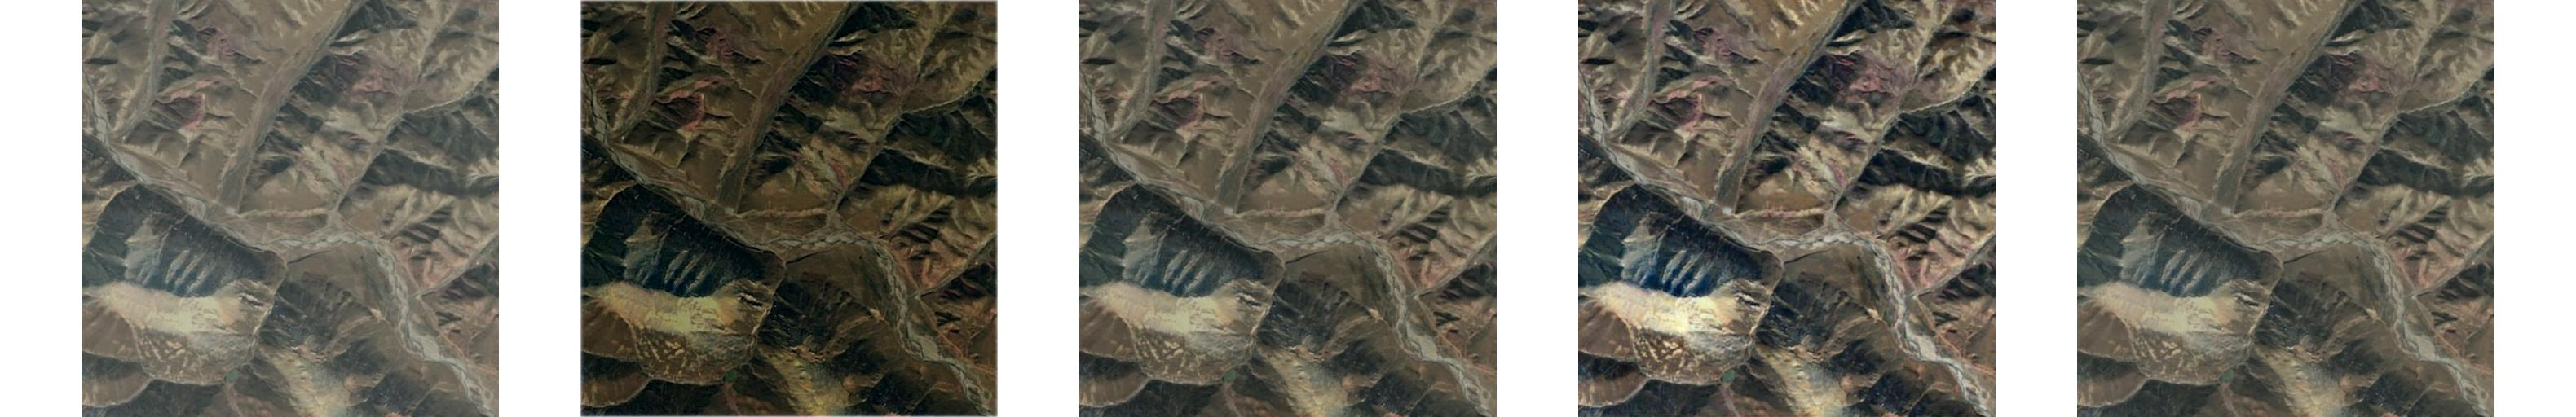
\includegraphics[width=14.5cm]{rice_3_1.jpg} \\
    Hazy Image\qquad\;\ AOD-Net\cite{li2017aod} \;\ GridDehazeNet\cite{liu2019griddehazenet} \;\; GCA-Net\cite{chen2019gated} \quad\; FFA-Net\cite{qin2020ffa}\\   
    
    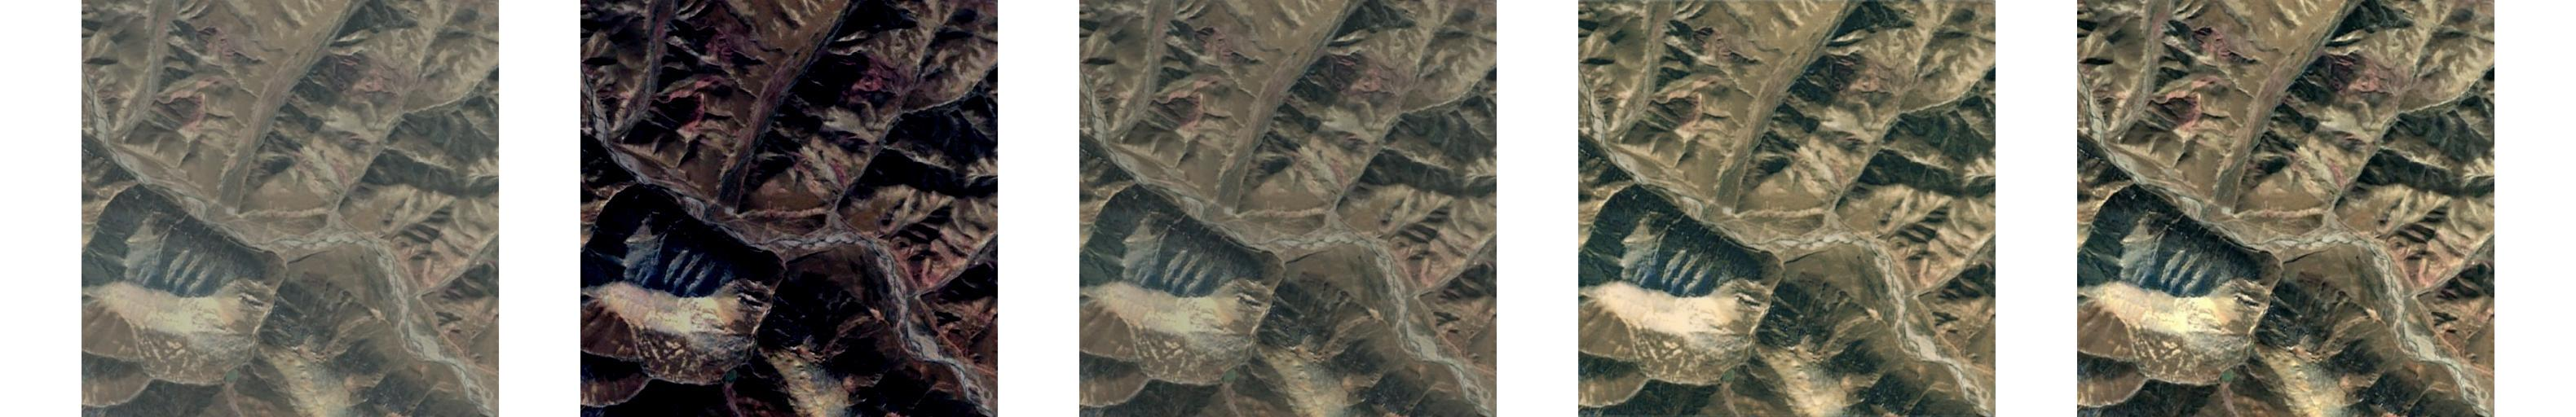
\includegraphics[width=14.5cm]{rice_3_2.jpg} \\
    MSBDN \cite{msbdn2020}\quad\quad\quad\, D4\cite{yang2022d4} \quad\quad DehazeFormer\cite{dehazeformer} \;\, Ours (LFD-Net) \quad\, Ground Truth \\   
    
    \caption{Visual Comparison Results on O-HAZE. We compare our methods with AOD-Net\cite{li2017aod}, GridDehazeNet\cite{liu2019griddehazenet}, Wavelet-U-Net\cite{yang2019wavelet}, GCA-Net\cite{chen2019gated}, FFA-Net\cite{qin2020ffa}, LD-Net\cite{ullah2021light} and D4\cite{yang2022d4}. AOD-Net and LD-Net produce relatively dark in visual quality. GCA-Net performs well on irregular haze but suffers from inconsistency in color blocks. Our proposed method exhibits adaptability to diverse scenarios and possesses a noteworthy level of generalization. }
    \label{rice}
\end{figure*}

\begin{figure*}[pht]
    \centering
    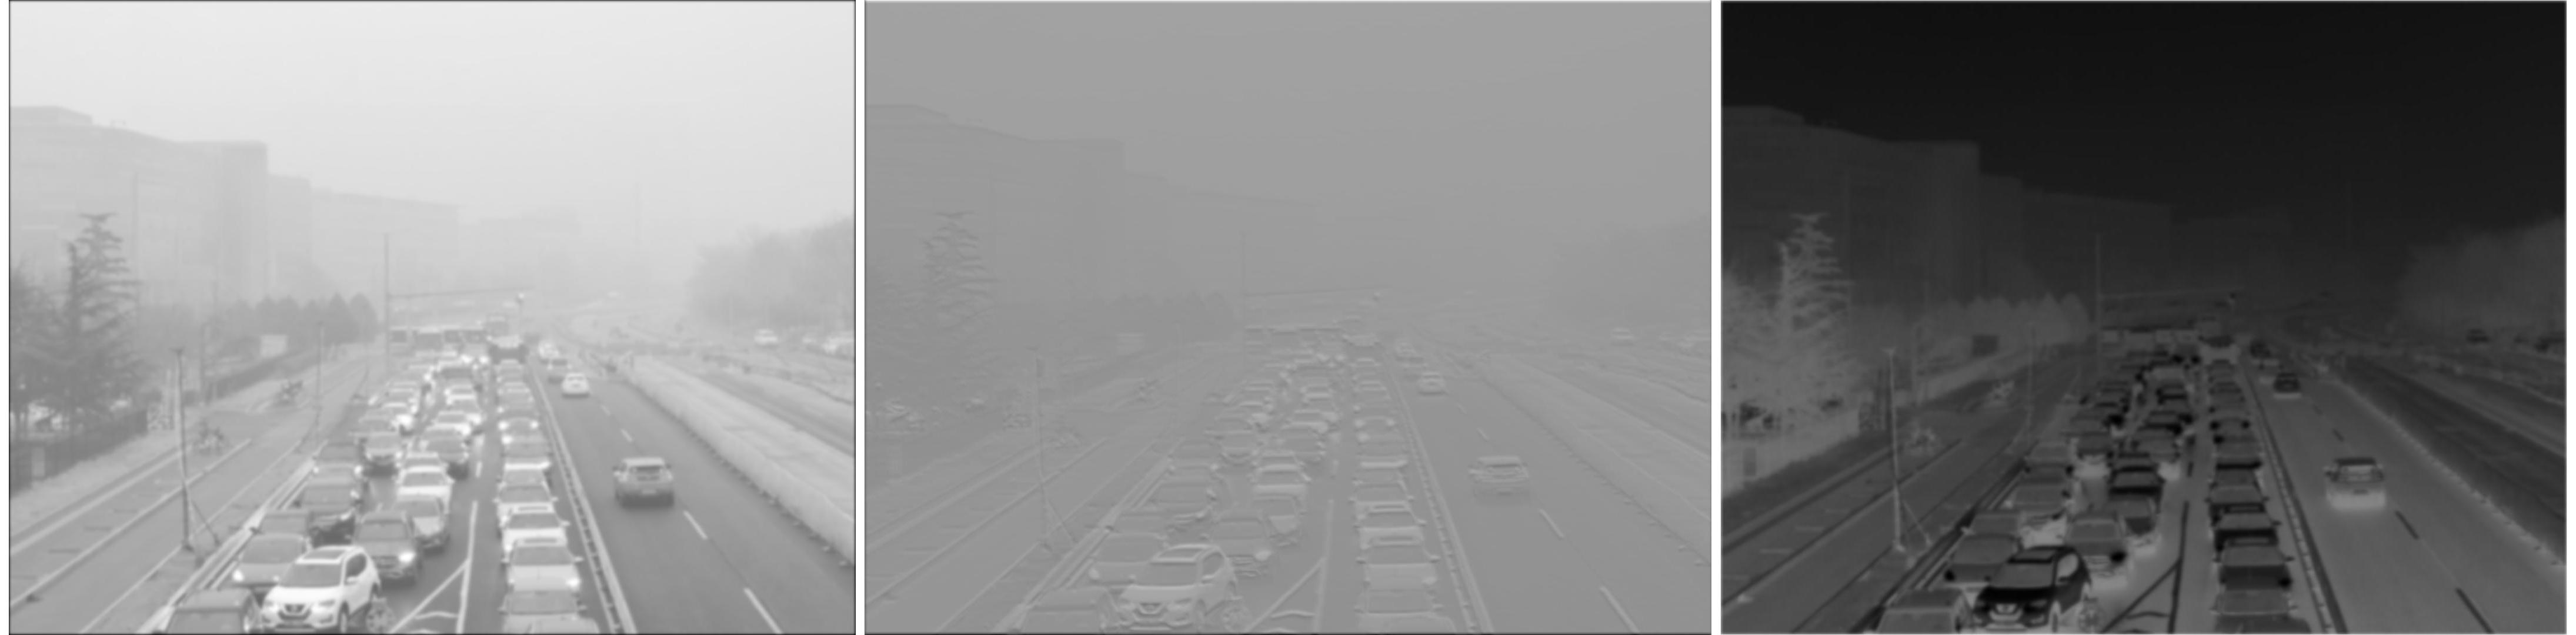
\includegraphics[width=\textwidth]{visual.jpg}
    The 1st Output Map of \textit{Conv 4} \qquad\qquad The 2nd Output Map of \textit{Conv 4} \qquad\qquad The 3rd Output Map of \textit{Conv 4} \\

    \quad \\
    
    (a) The Output of Convolutional Operation in Gated Fusion Module

    \quad \\
    %\caption{Visualization Results of the intermediate layers of Gated Fusion Module.}

    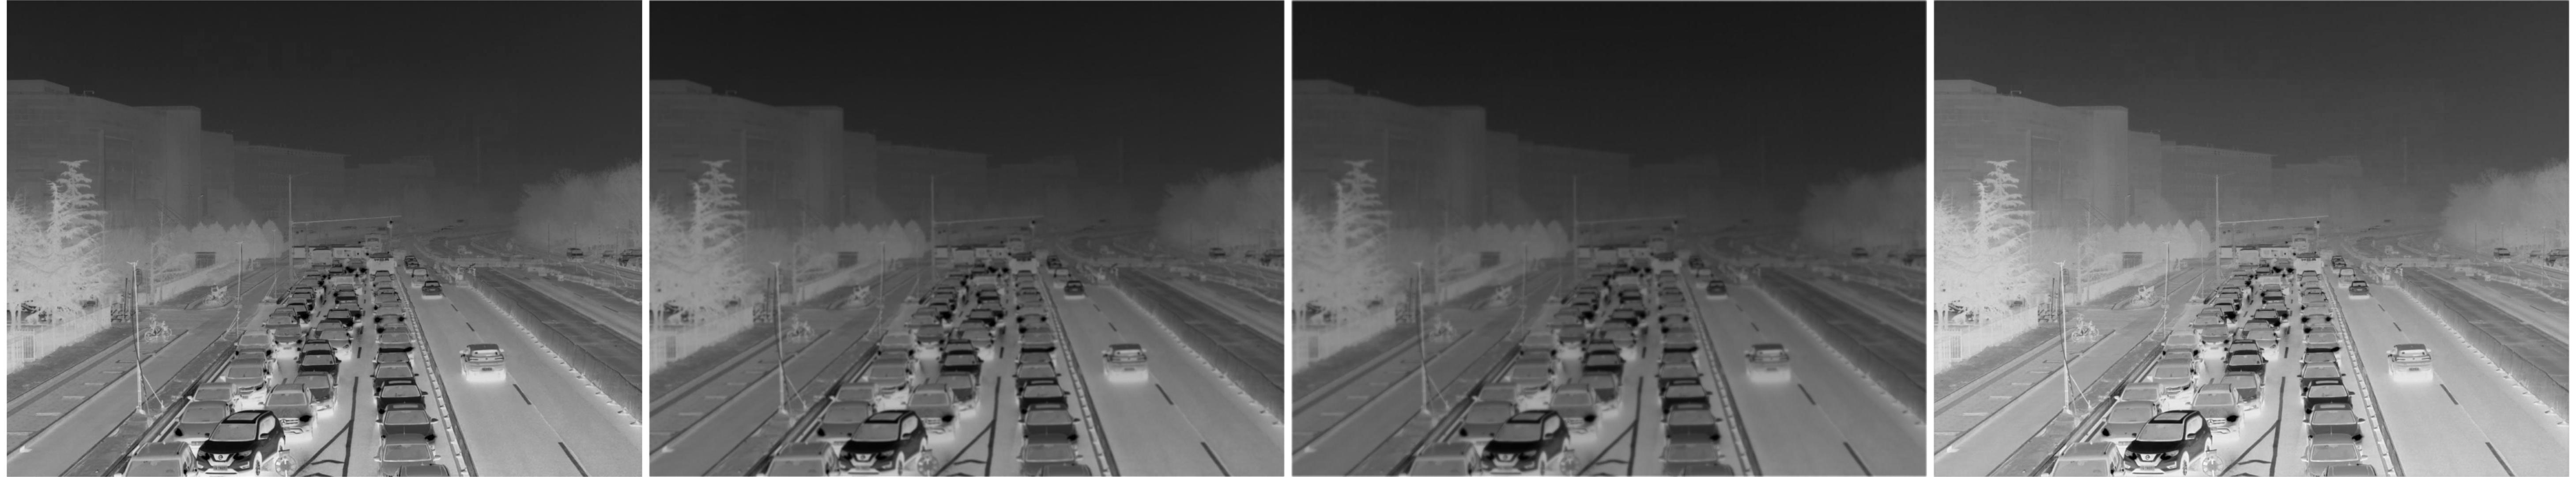
\includegraphics[width=\textwidth]{res15.jpg}
    The 1st Level of \textit{Concat 1} \quad The 2nd Level of \textit{Concat 1} \quad The 3rd Level of \textit{Concat 1} \quad\;\;\; Output of Gated Fusion\\

    \quad \\
    
    (b) The 15th Feature Map of Each Level of \textit{Concat 1} and the Output of Gated Fusion Module

    \quad \\
    
    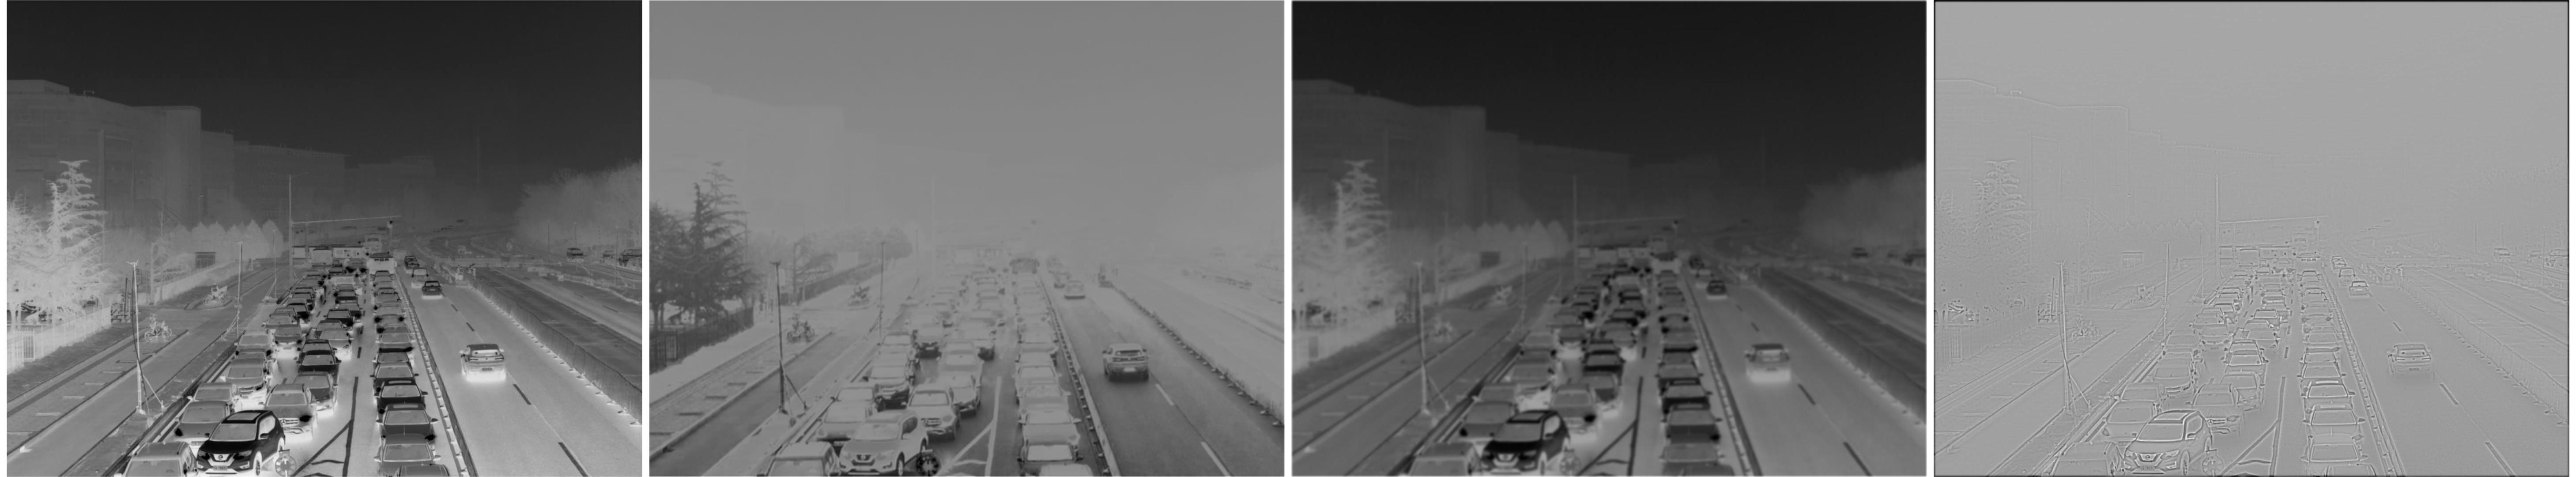
\includegraphics[width=\textwidth]{res30.jpg}
    The 1st Level of \textit{Concat 1} \quad The 2nd Level of \textit{Concat 1} \quad The 3rd Level of \textit{Concat 1} \quad\;\;\; Output of Gated Fusion\\

    \quad \\
    
    (c) The 30th Feature Map of Each Level of \textit{Concat 1} and the Output of Gated Fusion Module

    \quad \\
    
    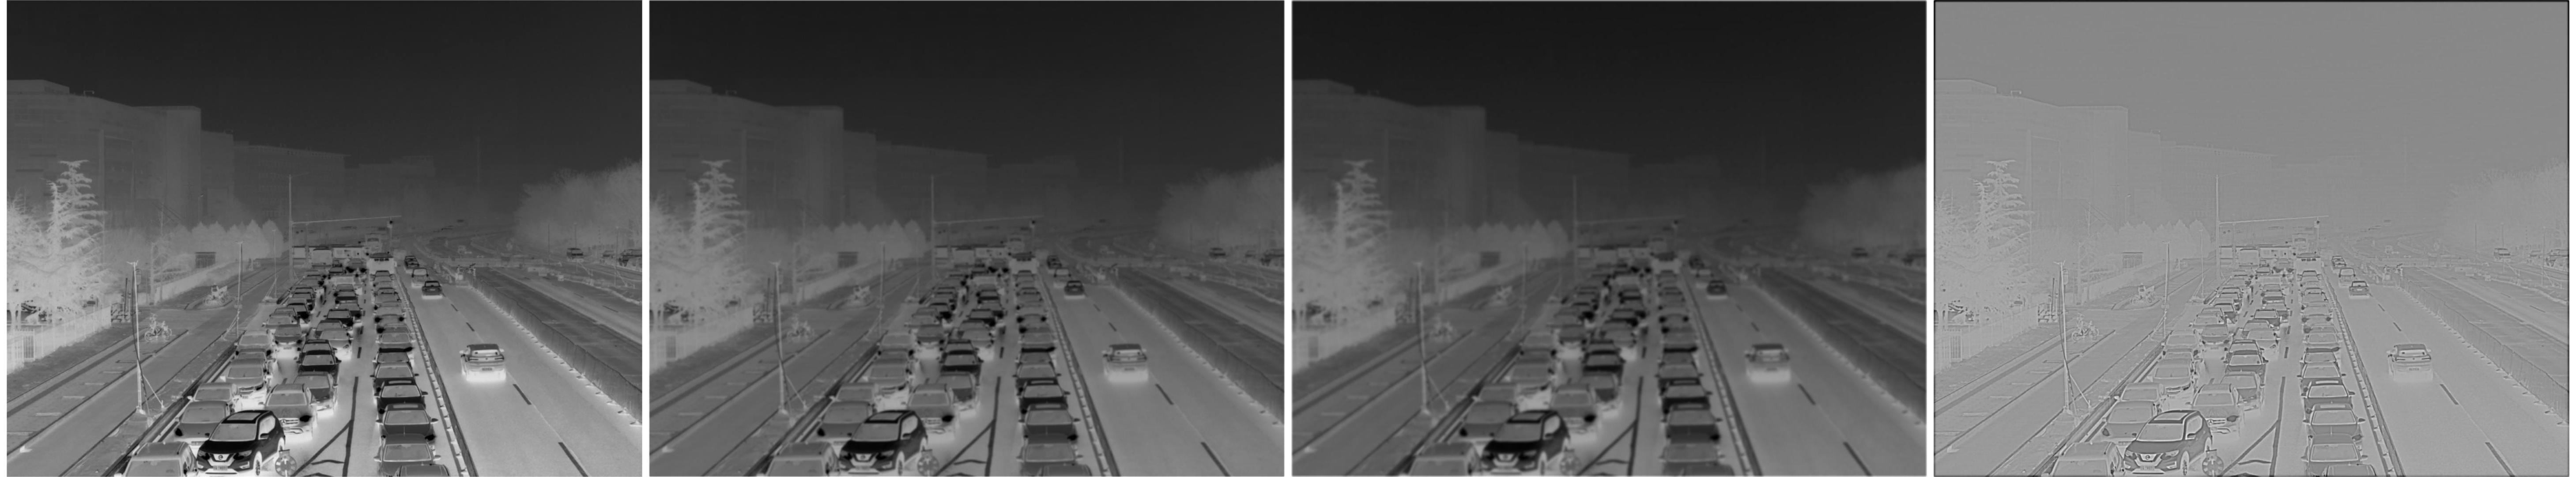
\includegraphics[width=\textwidth]{res31.jpg}
    The 1st Level of \textit{Concat 1} \quad The 2nd Level of \textit{Concat 1} \quad The 3rd Level of \textit{Concat 1} \quad\;\;\; Output of Gated Fusion\\

    \quad \\
    
    (d) The 31st Feature Map of Each Level of \textit{Concat 1} and the Output of Gated Fusion Module

    \quad \\
    
    \caption{Visualization Results of the changes in layers before and after the Gated Fusion Module: (a) represents the three output feature maps of the convolutional operation \textit{Conv 4} incorporated into Gated Fusion module, (b)-(d) stand for the changes in the 15th, 30th and 31st feature map of the layers respectively. (b) shows that the contrast of the image is enhanced, resulting in distant objects becoming more distinct. (c) and (d) show more abstract feature representations, which are significantly shifted compared to the input. Specifically, (c) emphasizes the outline of substances, while (d) highlights the blocks within substances.}
    \label{visual}
\end{figure*}
    
\begin{figure*}[pht]
    \centering
    
    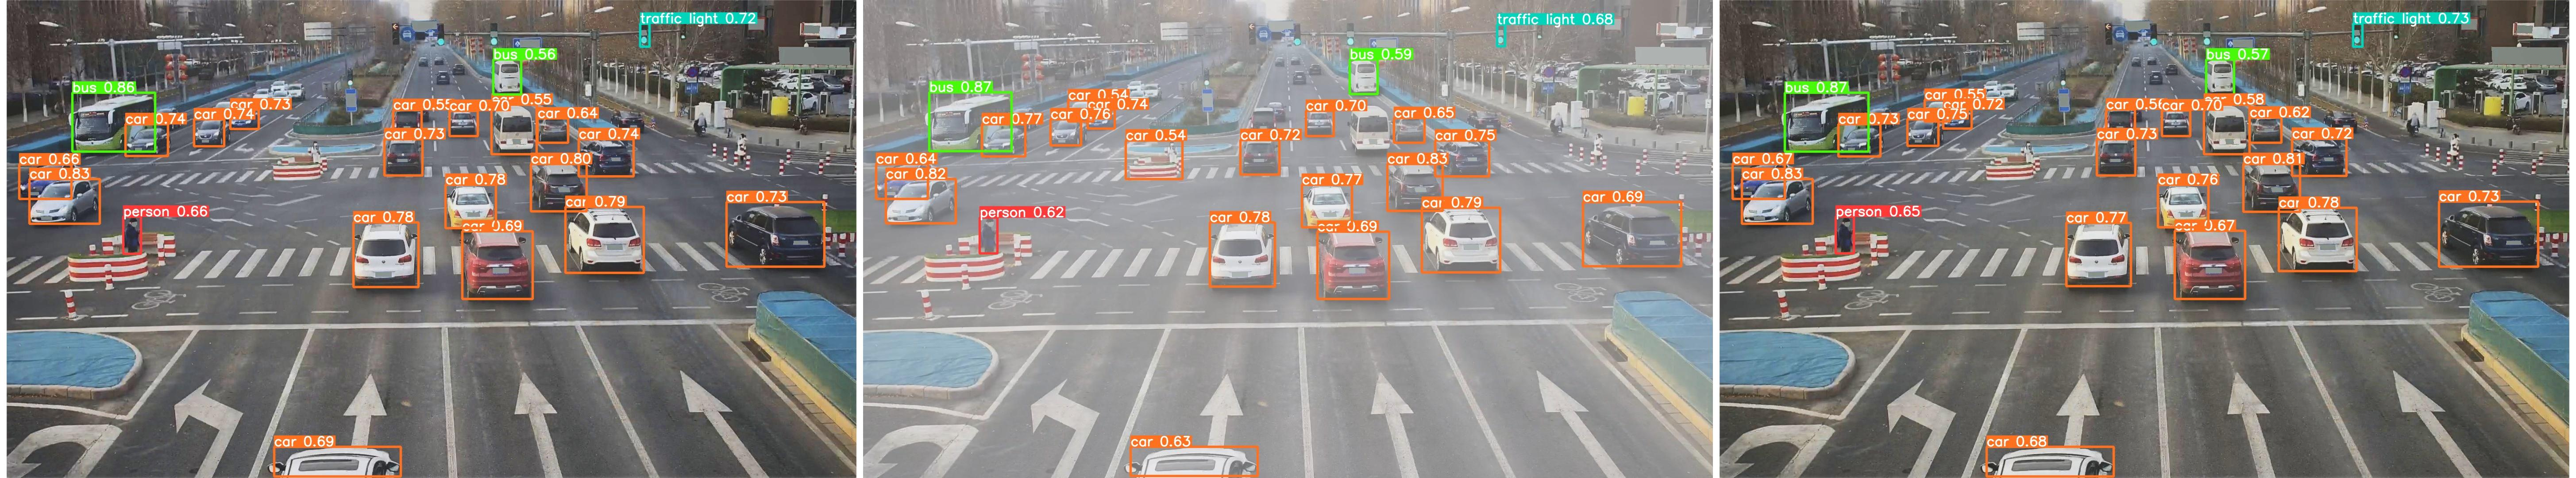
\includegraphics[width=\textwidth]{pic2.jpg}
    %\textit{(i)} \qquad \qquad \qquad \qquad \qquad \qquad \qquad \qquad \textit{(ii)} \qquad \qquad \qquad \qquad \qquad \qquad \qquad \qquad \textit{(iii)}\\
    Ordinary \qquad\qquad\qquad\qquad\qquad\qquad\qquad\quad Hazy \qquad\qquad\qquad\qquad\qquad\qquad\qquad Dehazed \\

    \quad \\
    
    (a) Comparison of Object Detection Results Under Different Conditions from DAIR-V2X\\

    \quad \\
    
    \includegraphics[width=\textwidth]{pic3.jpg}
    Ordinary \qquad\qquad\quad\, Hazy \qquad\qquad\quad\ Dehazed 
    \qquad \qquad \,
    Ordinary \qquad\qquad\quad\, Hazy \qquad\qquad\quad\ Dehazed\\

    \quad \\
    
    (b) \qquad\qquad\qquad\qquad\qquad\qquad\qquad\qquad\qquad\qquad\qquad\qquad\quad (c) \\

    \quad \\

    \includegraphics[width=\textwidth]{pic4.jpg}
    Ordinary \qquad\qquad\quad Hazy \qquad\qquad\quad\ Dehazing 
    \qquad \qquad \quad
    Ordinary \qquad\qquad\quad Hazy \qquad\qquad\quad\ Dehazing\\
    
    \quad \\
    
    (d) \qquad\qquad\qquad\qquad\qquad\qquad\qquad\qquad\qquad\qquad\qquad\qquad\quad (e) \\

    \quad \\
    
    \caption{Reference Object Detection Results: (a) comparison of object detection results under ordinary, simulated hazy, and dehazed conditions, (b)-(e) detailed sub-scenes of detection results \textcolor{blue}{under different conditions}. \textcolor{blue}{(b) and (c) demonstrate an improvement in the detection rate, detecting an additional car instance in the dehazed condition compared to the hazy condition.} (d) corrects the error of mistaking a roadblock for a car in the hazy condition. (e) shows the detection of another car compared to the ground-truth clear image.}
    
    \label{object_detection}
    
\end{figure*}

\begin{figure*}[pht]
    \centering    
    \includegraphics[width=\textwidth]{rm_pic2.jpg}
    Ordinary \qquad\qquad\qquad\qquad\qquad\qquad\qquad\quad Hazy \qquad\qquad\qquad\qquad\qquad\qquad\qquad Dehazed \\

    \quad \\
    
    (a) Comparison of Object Detection Results Under Different Conditions from VisDrone2019\\

    \quad \\
    
    \includegraphics[width=\textwidth]{rm_pic3.jpg}
    Ordinary \qquad\qquad\quad\, Hazy \qquad\qquad\quad\ Dehazed 
    \qquad \qquad \,
    Ordinary \qquad\qquad\quad\, Hazy \qquad\qquad\quad\ Dehazed\\

    \quad \\
    
    (b) \qquad\qquad\qquad\qquad\qquad\qquad\qquad\qquad\qquad\qquad\qquad\qquad\quad (c) \\

    \quad \\

    \includegraphics[width=\textwidth]{rm_pic4.jpg}
    Ordinary \qquad\qquad\quad Hazy \qquad\qquad\quad\ Dehazing 
    \qquad \qquad \quad
    Ordinary \qquad\qquad\quad Hazy \qquad\qquad\quad\ Dehazing\\
    
    \quad \\
    
    (d) \qquad\qquad\qquad\qquad\qquad\qquad\qquad\qquad\qquad\qquad\qquad\qquad\quad (e) \\

    \quad \\
    
    \caption{Reference Remote Sensing Object Detection Results: (a) comparison of remote sensing object detection results under ordinary, simulated hazy, and dehazed conditions, (b)-(e) detailed sub-scenes of detection results \textcolor{blue}{under different conditions}, in which the detection rate for pedestrians is enhanced to a large extent. In particular, (b) and (e) highlight instances of pedestrians that are not visible in the ordinary conditions but are detected after dehazing, similar to the results from DAIR-V2X.}
    
    \label{remote_object_detection}
    
\end{figure*}

In the remote sensing domain, to the best of our knowledge, pre-trained models for dehazing methods are not publicly available. However, we also reproduce 7 SOTA methods using default outdoor weights, including AOD-Net\cite{li2017aod}, GridDehazeNet\cite{liu2019griddehazenet}, GCA-Net\cite{chen2019gated}, FFA-Net\cite{qin2020ffa}, MSBDN\cite{msbdn2020}, D4\cite{yang2022d4} and DehazeFormer\cite{dehazeformer}. As expected, the performance of AOD-Net is limited due to its small number of parameters, while the other methods show similar performance before fine-tuning. In this paper, our pretrained model is open to the public for further comparison.

\textcolor{blue}{To demonstrate the effectiveness and efficiency of our proposed method, we present a comprehensive comparison using various metrics including PSNR, SSIM, CIEDE2000, $\Delta$SSEQ, and FPS. The comparison results are summarized in Tables \ref{tab:sots}, \ref{tab:ohaze}, and \ref{tab:rice}. Additionally, we provide a comparison of model sizes in Table \ref{tab:model_size}.}

\begin{table}[H]
    \caption{Average Comparison of Metrics on SOTS for 492 JPG Images\label{tab:sots}}
    \centering
    \begin{tabular}{cccccc}
    \hline
    &PSNR$\uparrow$ & SSIM$\uparrow$ & CIEDE$\downarrow$ & $\Delta$SSEQ $\downarrow$ & FPS$\uparrow$ \\
    \hline
    AOD-Net                 & 19.45 & 0.8593 & 7.12 & 0.0080 & \textbf{56.85} \\
    GridDehazeNet           & \underline{25.07} & \textbf{0.9108} & \textbf{4.02} & 0.0074 & 10.04 \\
    Wavelet-U-Net           & 23.73 & 0.8661 & 4.93 & 0.0064 &  8.28 \\
    GCA-Net                 & 22.13 & 0.8766 & 6.19 & \underline{0.0058} & 23.01 \\    
    FFA-Net                 & 19.36 & 0.8472 & 7.70 & 0.0131 &  6.91 \\
    LD-Net                  & 18.62 & 0.8380 & 7.52 & 0.0075 & 45.44 \\
    D4                      & 18.09 & 0.6668 & 8.36 & 0.0624 & 44.79 \\
    LFD-Net                 & \textbf{25.12} & \underline{0.9087} & \underline{4.24} & \textbf{0.0054} & \underline{54.41} \\
    \hline
    \end{tabular}
\end{table}

\begin{table}[H]
    \caption{Average Comparison of Metrics on O-HAZE for 45 JPG Images\label{tab:ohaze}}
    \centering
    \begin{tabular}{cccccc}
    \hline
    &PSNR$\uparrow$ & SSIM$\uparrow$ & CIEDE$\downarrow$ & $\Delta$SSEQ $\downarrow$ & FPS$\uparrow$ \\
    \hline
    AOD-Net        & 15.06 & 0.5412 & 17.53 & 0.0146 & \underline{13.93} \\
    GridDehazeNet  & 16.68 & 0.6361 & \underline{13.54} & 0.0055 & 1.09 \\
    Wavelet-U-Net  & 15.87 & 0.5058 & 14.93 & \textbf{0.0041} & 8.66\\
    GCA-Net        & \underline{17.24} & \underline{0.6523} & 13.81 & 0.0077 & 4.92 \\    
    FFA-Net        & 14.62 & 0.5881 & 14.72 & 0.0067 & 1.52\\
    LD-Net         & 14.72 & 0.5583 & 16.74 & 0.0057 & 10.62 \\
    D4             & 11.51 & 0.2564 & 18.58 & 0.1612 & 2.70 \\
    LFD-Net        & \textbf{17.67} & \textbf{0.6532} & \textbf{11.80} & \textbf{0.0041} & \textbf{14.65}\\
    \hline
    \end{tabular}
\end{table}

\begin{table}[H]
    \caption{Average Comparison of Metrics on RICE1 for 500 PNG Images\label{tab:rice}}
    \centering
    \begin{tabular}{cccccc}
    \hline
    &PSNR$\uparrow$ & SSIM$\uparrow$ & CIEDE$\downarrow$ & $\Delta$SSEQ $\downarrow$ & FPS$\uparrow$ \\
    \hline
    AOD-Net       & 14.80 & 0.6578 & 16.73 & 0.0508 & \textbf{58.62} \\
    GridDehazeNet & 19.14 & 0.8351 & 11.44 & 0.0021 & 5.08 \\
    %W-U-Net       & 23.46 & 0.8553 & & &  8.28\\
    GCA-Net       & 18.35 & 0.7237 & 15.25 & 0.0075 & 23.61 \\    
    FFA-Net       & 19.92 & 0.8117 & \underline{10.39} & 0.0029 & 7.06 \\
    MSBDN         & 19.77 & 0.8477 & 10.65 & 0.0022 & 21.38 \\ % \cite{msbdn2020}
    %LD-Net        & 18.63 & 0.8380 & & & 45.60\\
    D4            & 19.29 & 0.8258 & 12.21 & 0.0202 & 15.59\\
    DehazeFormer  & \underline{19.95} & \underline{0.8615} & 10.82 & \underline{0.0018} & 4.29 \\ % \cite{dehazeformer}
    LFD-Net       & \textbf{30.88} & \textbf{0.9420} & \textbf{3.32} & \textbf{0.0008} & \underline{45.51} \\
    \hline
    \end{tabular}
\end{table}

Observations reveal that many networks suffer from inconsistencies within color blocks or misrepresenting original information, as reflected in terms of CIEDE2000 and $\Delta$SSEQ. For instance, lightweight methods such as AOD-Net \cite{li2017aod}, LD-Net \cite{ullah2021light}, and D4 \cite{yang2022d4} produce relatively dark visual quality, resulting in a significant loss of texture information and making it difficult to distinguish objects for downstream tasks. While GCA-Net \cite{chen2019gated} encounters severe color shift occasionally in the synthetic SOTS dataset, it performs well in realistic scenarios like O-HAZE, which has thick and irregular haze. However, its halo effects and color imbalances are magnified in RICE1, which makes it less adaptive to generalized scenarios. FFA-Net \cite{qin2020ffa} performs well on specific datasets but distinctly lacks dehazing capability on RICE1, where there are a variety of landforms and terrains, rendering it not generalizable enough for shifted domains. 

\textcolor{blue}{From the experiment, we can observe that} incorporating attention mechanisms may prevent the image from being uniformly dehazed without region discrepancy (\textit{i.e.} FFA-Net) compared to networks with absolute convolutional and concatenation layers (\textit{i.e.} AOD-Net, LD-Net). However, a stack of sophisticated modules incorporating attention mechanisms may also confuse the model when selecting regions of interest, leading to insufficient attention paid to each hazy region and overfitting on specific datasets with limited data diversity, rendering these approaches not flexible enough for real-world vision tasks. 

Nevertheless, attention mechanisms are well adapted to U-Net or U-Net ensembling structures, where multi-scale features are addressed symmetrically. Wavelet-U-Net~\cite{yang2019wavelet} and GridDehazeNet~\cite{liu2019griddehazenet} have excellent performance, but they may come at the cost of inference time, \textcolor{blue}{6.6$\times$ and 5.4$\times$ longer compared to our proposed method, respectively.} Wavelet-U-Net transforms the image into the wavelet space using discrete wavelet transformation, which adds to the computational cost to some extent. GridDehazeNet also utilizes attention mechanisms but as a bridge of multi-scale features, which ensembles the design of U-Net~\cite{ronneberger2015u}. It has three rows and six columns, with each row corresponding to a different scale, constructing a grid network, which may compromise the inference speed. 

However, their performance on the HSTS dataset from \textcolor{blue}{Fig. \ref{hsts}} and randomly selected hazy images from \textcolor{blue}{Fig. \ref{own}} demonstrates that they may also suffer occasional degradation when dealing with remote objects that are occluded, as well as objects located in areas uniformly covered with thick haze but with limited prior semantic information. \textcolor{blue}{While the images randomly selected for our study in Fig. \ref{own} may not be representative of specific datasets, they are still valuable for consideration as they reflect scenarios that can occur in real-world practices. Although accurately verifying the generalization of algorithms is challenging, our approach has demonstrated effectiveness even when encountering severe domain shifts, as evidenced by our experiments.} Our proposed method does not adopt the U-Net structure for efficiency, nor does it leverage stacked attention mechanisms, which saves the computational cost to a large extent, exhibits adaptability to diverse scenarios, and possesses a noteworthy level of generalization.

\subsection{Ablation Study}

The experimental results confirm that our proposed LFD-Net is effective and efficient for real-time applications. Since it has a different principle than other methods, we perform a series of ablation studies to ensure that each component of the network is indispensable. The detailed experimental conditions and corresponding metrics tested on outdoor SOTS are listed in Table \ref{tab:ablation}. 

\begin{table*}[htpb]
    \caption{\textcolor{blue}{Comparison of the Parameters of Models}\label{tab:model_size}}
    \centering
    \begin{tabular}{ccccccccccc}
    \hline
      & AOD-Net & GridDehazeNet & Wavelet-U-Net & GCA-Net & FFA-Net & LD-Net & D4 & MSBDN & DehazeFormer & LFD-Net \\ 
    \hline
    Params($\times$M) & 0.002 & 0.956 & 11.3 & 0.702 & 4.46 & 0.030 & 10.7 & 28.7 & 2.51 & 0.086 \\
    \hline
    \end{tabular}
\end{table*}

\begin{table*}[hbtp]
    \caption{Ablation Experiment of LFD-Net on Outdoor SOTS Dataset\label{tab:ablation}}
    \centering
    \begin{tabular}{cccccccc}
    \hline
      &\textit{Concat 2} & Gated Fusion Module & Attention Mechanism & PSNR$\uparrow$ & SSIM$\uparrow$ & CIEDE$\downarrow$ & $\Delta$SSEQ $\downarrow$\\
    \hline
    Case 1 & \usym{1F5F4} &  &  & \underline{24.35} & \underline{0.9062} & \underline{5.09} & 
    \underline{0.0055} \\
    Case 2 &  & \usym{1F5F4} &  & 23.33 & 0.8910 & 5.56 & 0.0066 \\
    Case 3 &  &  & \usym{1F5F4} & 21.62 & 0.8642 & 6.65 & 0.0116 \\
    Case 4 &  & \usym{1F5F4} & \usym{1F5F4} & 23.17 & 0.8878 & 5.54 & 0.0076 \\
    %Case 5 & \multicolumn{3}{c}{\textit{Concat 1} - \textit{Conv 4} - \textit{Concat 2} - Gated Fusion Module - Attention Mechanism} & 22.43 & 0.8743 & & \\
    %Default & \multicolumn{3}{c}{\textit{Concat 1} - Gated Fusion Module - \textit{Concat 2} - Attention Mechanism} & \textbf{25.02} & \textbf{0.9122} & & \\
    Default & & & & \textbf{25.12} & \textbf{0.9087} & \textbf{4.24} & \textbf{0.0054} \\
    \hline
    \end{tabular}
\end{table*}

Inspired by \cite{li2017aod} and \cite{ullah2021light}, we add a second concatenation layer (\textit{i.e.} \textit{Concat 2}), to our method. In Case 1, we omit \textit{Concat 2} and observe a slight loss of detailed texture information due to the reduced high-level information. 

In Cases 2, 3, and 4, we investigate the importance of the Gated Fusion module or attention mechanism in our model. These cases demonstrate that these two sub-networks work together to facilitate feature interaction. Specifically, the removal of the attention mechanism leads to the occasional appearance of black spots on the images, which significantly degrades the overall performance. In comparison with other lightweight methods, our method partially addresses this issue. Additionally, the Gated Fusion module is a crucial component in enhancing the dehazing capability, serving as a bridge between the multi-level feature extraction process, which ends at the first concatenation layer \textit{Concat 1}, and the attention mechanism, which begins at the second concatenation layer \textit{Concat 2}. 

When both the attention mechanism and the Gated Fusion module are involved, the detailed information in the images is further refined, making it more authentic and faithful to the original information. This structure helps to preserve and interact with multi-level information to improve the overall image quality.  

\subsection{Visualization Results}
We have visualized the intermediate feature maps before and after the Gated Fusion Module, as  depicted in Fig. \ref{visual}. As shown in (a), the incorporated convolutional layer combines features of three levels from \textit{Conv 1}, \textit{Conv 2} and \textit{Conv 1 + Conv 3} to generate three distinctive feature maps. They are distinguished from each other by their focus on close or distant objects and the lightness or contrast of the pixels. 

In Fig. \ref{visual} (b)-(d), we demonstrate the changes in specific feature maps after the Gated Fusion module. Fig. \ref{visual} (b) shows that the contrast of the image is enhanced with the hierarchical information, resulting in distant objects becoming more distinct. Fig. \ref{visual} (c) and Fig. \ref{visual} (d) show more abstract feature representations, which are significantly shifted compared to the input features. Specifically, Fig. \ref{visual} (c) emphasizes the outline of substances, while Fig. \ref{visual} (d) highlights the blocks within substances.

The Gated Fusion module re-allocates the distributed feature representations of the multi-level layers through feature-interaction strategies. The feature extraction process is compressed into three successive convolutional layers, for which we compensate by intra-level enhancement and inter-level combination.  

\subsection{Application for Object Detection Task}
As a severe weather condition, haze can significantly reduce the effectiveness of remote sensing land obsevation system. For instance, object detection results in automatic driving applications suffer from hazy environments and may be put into risky situations due to the degradation of image quality. Therefore, pre-processing procedure for image enhancement before performing those tasks is of great importance. As far as we know, there is no dataset with built-in synthetic fog images for object detection. In our experiment, we randomly select 100 images from each dataset (DAIR-V2X and VisDrone2019) and produce their synthetic hazy versions. We use the default outdoor pretrained weight for the former and the fine-tuned remote sensing pretrained weight for the latter. Both object detection processes are based on YOLOv5. Our experiment results show that the mean Average Precision when IoU = 0.5 (mAP@0.5) of the dehazed condition improves by 4.73\% compared to the hazy condition in DAIR-V2X, while by 0.81\% in VisDrone2019.

Furthermore, overall detection result of a particular scene is shown in Fig. \ref{object_detection} (a), while Fig. \ref{object_detection} (b)-(e) illustrate the most representative perspectives of the dehazing effect. In Fig. \ref{object_detection} (b) and (c), it can be seen that dehazing improves the detection rate, \textcolor{blue}{as an additional car instance is detected in the dehazed condition compared to the hazy condition.} In Fig. \ref{object_detection} (d), the roadblock is mistakenly identified as a car in the hazy condition, but the dehazing method is able to remove this error. In Fig. \ref{object_detection} (e), another car instance is shown before and after dehazing the synthetic hazed image. 

In Fig. \ref{remote_object_detection} (a), we show the overall remote sensing object detection results from the perspective of a drone in a particular scene. In the images captured by the drone, the types of land cover are more complex and the objects are smaller when compared to the driving perspective from DAIR-V2X. Fig. \ref{remote_object_detection} (b)-(e) illustrate the difficulties object detection methods encounter when detecting smaller pedestrian instances, especially in hazy conditions. However, dehazing methods can partially address this issue and enhance the detection rate of small objects like pedestrians, as shown in Fig. \ref{remote_object_detection} (c) and (d). In Fig. \ref{object_detection} (b) and (e), two additional pedestrian instances are detected after dehazing compared to the original conditions, similar to that in Fig. \ref{object_detection} (e). Experimental results show that haze can have unpredictable effects on normal conditions, and our method can provide a better solution compared to the ground truth in representing high-level semantic information to some extent.


\section{Conclusion}
In this paper, we propose a novel end-to-end model called LFD-Net for remote sensing image dehazing. As a pre-processing for downstream vision tasks, it not only ensures the effectiveness and efficiency required for real-time applications, but also outperforms SOTA methods in terms of region-balance and color-fidelity. By designing this framework, we demonstrate the potential of CNN-based networks by performing two-order spatial interaction. Specifically, we show that the capabilities of deep neural networks can be enhanced not only by adding more complex modules to be deeper, but also by effectively combining individual and natural feature extraction, fusion, and attention with feature interaction strategies, particularly in the field of image super-resolution. The experiments on various scenarios also shows that performance of a model is not always propotional to the number of parameters, and less parameters to some extent may help mitigate overfitting, which might be conducive for future network design.


\bibliographystyle{IEEEtran}
\bibliography{ref}
%\section{Biography Section}
\begin{IEEEbiography}[{\includegraphics[width=1in,height=1.25in,clip,keepaspectratio]{jyz.jpg}}]{Yizhu Jin} is currently a final year undergraduate student in the School of Automation Science and Electrical Engineering from Beihang University, Beijing, China. Jin's research interests lie in the intersection between valuable application and general methods with high interpretability in Computer Vision and Artificial Intelligence.  
\end{IEEEbiography}


\begin{IEEEbiography}[{\includegraphics[width=1in,height=1.25in,clip,keepaspectratio]{cjx.png}}]{Jiaxing Chen} received M.S. degree in Electrical and Computer Engineering from University of Illinois, Chicago, USA, in 2021 and worked as an Algorithm engineer in National Innovation Center of Intelligent and Connected Vehicles in 2022. He is currently a researcher with Tsinghua University, Beijing, China. Chen's research interests include Computer Vision with Deep Learning, Machine Learning, Multimodal Fusion, and Trajectory Prediction.
\end{IEEEbiography}

\begin{IEEEbiography}[{\includegraphics[width=1in,height=1.25in,clip,keepaspectratio]{tf.png}}]{Feng Tian} received her B.S. degree in engineering in 2018. She is currently studying in the College of Traffic and Logistics Engineering, Xinjiang Agricultural University, Xinjiang, China, pursuing a Postgraduate degree in transportation engineering. Tian's research interests include Machine Learning, Data Mining, Intelligent Transportation, and Target Detection.
\end{IEEEbiography}

\begin{IEEEbiography}[{\includegraphics[width=1in,height=1.25in,clip,keepaspectratio]{hk.png}}]{Kun Hu} received the B.Sc. degree in Remote Sensing Science and Technology from Wuhan University, Wuhan, China, in 2010, the M.Sc. and Ph.D. degree in Photogrammetry and Remote Sensing from Wuhan University in 2012 and 2016, respectively.

He worked as an assistant professor with the Institute of Electronics, Chinese Academy of Sciences, Beijing, China from 2012 to 2017, as a post-doctor with the Ohio State University, Ohio, USA, from 2017 to 2019, and as an associate professor with the Aerospace Information Research Institute, Chinese Academy of Sciences, Beijing, China from 2019 to 2022. 

He is currently an associate professor with the Institute of Artificial Intelligence, Beihang University, Beijing, China. His research interests focus on the accurate processing and intelligent application of multi-source remote sensing data, such as camera calibration, image production, information fusion, target detection, clarification, 3D reconstruction and quality evaluation. 

\end{IEEEbiography}


%\vspace{11pt}

%\bf{If you will not include a photo:}\vspace{-33pt}
%\begin{IEEEbiographynophoto}{John Doe}
%Use $\backslash${\tt{begin\{IEEEbiographynophoto\}}} and the author name as the argument followed %by the biography text.
%\end{IEEEbiographynophoto}
\end{document}